%======================================================================
%	Vorlage
%======================================================================
%	$Id$
%	Matthias Kupfer
%======================================================================
%	Documentclass
%======================================================================
\documentclass[
%	draft,			% Entwurfsmodus: Bilder als Rahmen,
				% Überlängen werden deutlich markiert
%	10pt,			% 
	11pt,			% KOMA default
%	12pt,			% 
	a4paper,		% DIN A4
%	twoside,		% Zweiseitig
%	german,			%
    % english
%----------------------------------------------------------------------
% Die folgenden Befehle stammen aus dem KOMA Paket
	% headsepline,		% Linie unter der Kopfzeile	
%	headnosepline,		%
%	foodsepline,		% Linie über Fussnote	
	footsepline=false,	%
	automark,		% Kolumnentitel lebendig
%	bigheadings,		% default: Überschriften gross setzen
	headings=normal,	% Überschriften normal setzen
%	smallheadings,		% Überschriften eher klein setzen
	pointlessnumbers,	% Keinen Punkt hinter die letzte Zahl 
				% eines Kapitels (auch bei Anhang)
%	chapterprefix,		% Kapiteluberschriften "Kapitel"
%	appendixprefix,		% Anhang
%	openright,		% Kapitel auf der rechten (ungeraden) Seite 
				% anfangen lassen
	openany,		% 
%	cleardoublestandard,	%
	cleardoublepage=plain,	%
%	cleardoubleempty,	%
	abstracton,		%
	index=totoc,		% Index soll im Inhaltsverzeichnis auftauchen
	listof=totoc,		%
	bibliography=totoc,	%
%	parskip, 		% parskip-, parskip*, parskip+
% 	halfparskip, 		% halfparskip-, halfparskip* und halfparskip+
%	DIVclassic,
% 	BCOR=8mm,		%%?? Bindungskorrektur: 
				% BCOR<Breite des Bindungsverlustes> 
]{scrreprt} 

%======================================================================
%	Bearbeitung sowohl mit LaTeX als auch mit pdfLaTeX ermoeglichen
%======================================================================
%\newif\ifpdf 
	%\ifx\pdfoutput\undefined 
	%\pdffalse 			% we are not running pdflatex 
%\else 
	%\pdfoutput=1 			% we are running pdflatex 
	%\pdftrue 
%\fi


%======================================================================
%	Verwendete Pakete
%======================================================================

%\usepackage{babel}		% Sprachen

%% Latex mit deutschen Umlauten:
%% http://www.cs.albany.edu/~herrmann/latex_umlaute/
\usepackage[T1]{fontenc}	% EC-Schriften verwenden (vs. DC) da 8-Bit
				% EC-Schriften als T1-kodierten CM-Schriften
				% European/Ext.-Computer-Modern-(EC)-Schriften
				% Umlaute, Anführungszeichen ...
				% => Umlauten koennen richtig getrennt werden
				% FAQ 5.3.2

%\usepackage{ucs}		% Eingabe von ü,ö,ä,ß mit UTF-8 erlaubt
%\usepackage[utf8]{inputenc}	% (auch in Include-Dateien)
				% ! Zeichensatz der Dateien als UTF-8 !
								
\usepackage{ae,aecompl}		% virtuelle-CM-Fonts
				% da EC nicht als PostScript-(Type-1) verfuegbar
				% => keine echten Umlaute im PDF-Dokumen 
				%(Problem bei Suche)
				% By loading the ae package (\usepackage{ae}), 
				% you loose some characters as mentioned in 
				% README. 
				% The package aecompl by Denis Roegel restores
				% these characters which are taken from the ec 
				% fonts. If you use pdftex, you will get these 
				% characters as bitmaps, but this might be 
				% better than not having them at all.
\usepackage{bbold}
\usepackage{amsmath}
\usepackage[hang]{caption}
%\usepackage{times, mathptm}	% TimesNewRoman Schrift (Acrobat Reader Fonts), 
				% dazu braucht man auch den entsprechenden 
				% Zeichensatz für den Math-Mode
%\usepackage{pslatex}		% ? mathematische Formeln mit Standard 
				% Postscript Fonts gesetzt
			% Paket     Roman         Serifenlos  Typewriter
%\usepackage{times}	% -----------------------------------------------
			% times     Times         Helvetica   Courier
			% palatino  Palatino      Helvetica   Courier
			% newcent   NewCenturySch AvantGarde  Courier
			% bookman   Bookman       AvantGarde  Courier
			% Diese Schriften sind die Standard-PostScript-Schriften
			% und in jedem Drucker verfügbar

\usepackage{
%	german,			% Deutsche Trennungen (ALTE Rechtschreibung), 
				% Anführungsstriche und mehr 
%	ngerman,		% Deutsche Trennungen (NEUE Rechtschreibung), 
				% Anführungsstriche und mehr
				%
%	acronym,		% Verwaltung von Abkuerzungen
%	bibgerm,		% Deutsche Bibliographie 
	calc,			% Erweiterung der arithmetischen Funktionen in 
				% LaTeX
				% wird verwendet um Titelseite zu zentrieren
	color,			% im Laufenden Text einfach mit \color{Farbe) zwischen den 
				% Farben umschalten, wobei Farbe einfach 
				% durch z.B. red, blue, black etc. ersetzt wird
				% \textcolor{farbe){Text)
	datetime,   % definiere Datumsstile
	enumitem,   % mehr Optionen für enumerate environments 
%	epigraph,		% Zitat am Kapitelanfang
%	fancyhdr,		% Kopf- und Fußzeilen von Dokumenten frei 
				% gestalten
	fancybox,		% shadowbox, doublebox, ovalbox, Ovalbox 
	fancyvrb,		% verbatim Erweiterung:
	%glossary,		% Glossar und Abkürzungsverzeichnis
	mdwlist,		% compact list: itemize* ..
	scrdate,		% \todaysname 
	scrtime,		% \thistime
	scrlayer-scrpage,		% Kopf- und Fußzeilen flexibel gestalten
				%
%	moreverb,		% verbatim-ähnlich: boxedverbatim, listing
%	verbatim,		% Darstellung von "Text, wie er eingegeben wird"
				%
%	lscape,			% Erstellt eine um 90% gedrehte *neue* Seite
%	textcomp,		% Sonderzeichen
%	booktabs,		% Tabellenlinien
%	longtable,		% Tabellen > 1 Seite
%	supertabular,		% Tabellen > 1 Seite
	tabularx,		% Blocksatzspalten
%	ltxtable,		% tabularx + longtable
%	multicol,		% mehrspaltige Zeilen
%	varioref,		% einheitliche Verweise
%	endnotes,		% Fussnoten -> Endnoten
%	rotating,		% sidewaystable und sidewaysfigure
%	natbib,			% Bibliographie ohne Klammer etc.
%	marvosym,		% Euro etc.
	tikz,
	pgf-umlsd,
	scrhack,
}
\usetikzlibrary{shapes.geometric, arrows, positioning}

\usepackage[acronym,toc]{glossaries}
\makeglossaries


\usepackage{listings}

%\usepackage{pstricks}
%\usepackage{listings}
%\usepackage{wasysym}

%\usepackage[german, first, bottomafter]{draftcopy}

%\usepackage{setspace}	% Durchschuß, Zeilenabstand
%\doublespace		% doppelzeilig oder
%\onehalfspacing	% anderthalbzeilig
\renewcommand{\baselinestretch}{1.1}\normalsize

% Für schöne Darstellung von Algorithmen
%\usepackage[german, algoruled, algochapter]{algorithm2e}
%\usepackage{algorithmic}
%\usepackage[chapter]{algorithm}

%======================================================================
%	Pictures, Links
%======================================================================

\usepackage{graphicx}
\graphicspath{Pictures/}	% Angabe der Pfade, wo die Grafiken liegen; 
				% mehrere Pfade sind möglich
\usepackage{subfig}
\usepackage{thumbpdf}
\usepackage[breaklinks]{hyperref}
\def\UrlBreaks{\do\/\do-}
%\usepackage{breakurl}
%\usepackage{minted}


%======================================================================
%	Added by me
%======================================================================

% \usepackage[backend=biber, style=user]{biblatex}
% \addbibresource{literature.bib} 

%======================================================================
%	user.sty
%======================================================================

\usepackage{user}	% Makros in user.sty 
			% \epsinc{bild.eps}{scale=1}{Bildunterschrift}
			% \missing{Beweis fehlt noch}
			% \comment{Ein Kommentar}

%======================================================================
%	Settings
%======================================================================

%\typearea{11}		% Satzspiegel neu konstruieren (KOMA)
			%      10pt 11pt 12pt 
			% DIV : 8   10   12  

\pagestyle{scrheadings}	% Standart  Kopf- und Fußzeile
\setkomafont{pageheadfoot}{\small\scshape}

% ---------------------------------------------------------------------
%\setcounter{secnumdepth}{2}
%\setcounter{chapter}{-1}
\setcounter{tocdepth}{3}

% ---------------------------------------------------------------------
%\sloppy		% weniger Worttrennungen, größere Wortabstände
\fussy			% viele Worttrennungen, "schönere" Wortabstände

% ---------------------------------------------------------------------
%\flushbottom			% Ausrichtung der Seitenenden jeweils auf 
				% gleicher Höhe

% ---------------------------------------------------------------------
%\sloppypar		% Das hier relaxt die Einstellungen zum Wortabstand 
			% extrem. Damit ragen keine Worte über den rechten 
			% Zeilenabstand hinaus. Dafür muß stärker auf
			% Wortabstand geachtet werden, der kann dann ziemlich 
			% groß werden. Man erhält aber keine Meldung mehr 
			% über underfull boxes.

%Hiermit kann man das gleiche mit weniger Holzhammer erreichen:
%\setlength{\tolerance}{2000}           % Strafpunkt für Zeilenumbruch
%\setlength{\emergencystretch}{3pt}     % Soweit dürfen einzelne Worte mehr 
					% auseinandergezogen werden
%\setlength{\hfuzz}{1pt}                % Macht den rechten Rand um bis zu 1pt 
					% flatterig.

% ---------------------------------------------------------------------
%Vermeiden einzelner Zeilen am Ende einer Seite oder oben auf einer neuen Seite
%\clubpenalty10000
%\widowpenalty10000

% ----------------------------------------------------------------------
% neue Umgebungen für verwendete Sätze und Beispiele
\newtheorem{bsp}{Beispiel}[chapter]
\newtheorem{satz}{Satz}[chapter]

% Eigene Anpassungen
% Silbentrennung
\tolerance 1414
\hbadness 1414                                                                  \emergencystretch 1.5em
\hfuzz 0.3pt
\widowpenalty=10000
\hyphenpenalty=200
\clubpenalty = 10000
\widowpenalty = 10000
\displaywidowpenalty = 10000
\vfuzz \hfuzz
\raggedbottom


%======================================================================
%	includeonly
%======================================================================

\includeonly{		% Shows which file shall be included by the include command
		%
  metadata		% set in variables
  ,title		% title page, Summary and table of contents
% All files for the include command have to be listed here!
  ,Text/01.Introduction	%
  ,Text/02.Fundamentals
  ,Text/03.Implementation
  ,Text/04.Results
  ,Text/05.Evaluation
  ,Text/06.Summary_Outlook
}

% Recommended structure of your scientific work
%
% Title Page
% Bibliographic Description (Backside of Title Page)
% (Task)
% Acknowledgement
% Abstract
% Table of Contents
% List of Tables
% List of Figures
% Introduction
% Content
% Summary/Outlook
% (List of used terms)
% Glossary (List of Abbreviations)
% (Index)
% Bibliography/References
% (Theses)
% (Declaration of Authorship)
% Attachments


%======================================================================
% * *   T E X T    S T A R T S    H E R E   * * * * * * * * * * * * * *
%======================================================================

\begin{document}
%======================================================================
%	Metadata
%======================================================================
%	$Id$
%	Matthias Kupfer
%======================================================================

\newcommand{\dcsubject}{Master Thesis}
% z.B. (Diplom/Studien/Haus)arbeit, Praktikumsbericht, Studie, Beleg, 
% (Pro/Haupt/Ober)seminar, Seminar usw.
\newcommand{\dctitle}{System Design, Implementation and Evaluation of a User-centered Application for Indoor Sound Classification}
\newcommand{\dcsubtitle}{~} % Subtitle, if necessary

\newcommand{\dcauthorlastname}{Sun}
\newcommand{\dcauthorfirstname}{Maoyin}
\newcommand{\dcauthoremail}{maoyin.sun@s2016.tu-chemnitz.de}
\newdateformat{mydate}{{\THEDAY} \monthname[\THEMONTH] \THEYEAR}
\newcommand{\dcdate}{\mydate\today}
%\newcommand{\dcdate}{\today}

\newcommand{\dcplace}{Chemnitz} % Ort, kann an der TU meist so bleiben
\newcommand{\dcuni}{Technische Universität \dcplace}
\newcommand{\dcdepart}{Faculty of Computer Science} % Fakultätsangabe
\newcommand{\dcprof}{Junior Professorship of Media Computing} % Angabe der Professur

\newcommand{\dcpruefer}{Jun.-Prof. Dr. rer. nat. Danny Kowerko}% Prüfer der Arbeit
\newcommand{\dcadvisor}{M. Sc. Arunodhayan Sampath-Kumar}% Betreuer der Arbeit

\newcommand{\dckeywords}{System Design, User-centered Application, Indoor Sound Classification, Web-based Demonstration Platform, Asynchronous Messaging, Acoustic Event Classification, Decoupled Architecture, MQTT, D3.js, Real-time Streaming}

%%======================================================================
% Settings of Hyperref-Package
\hypersetup{%    
    pdftitle	= {\dctitle}, %
    pdfsubject	= {\dcsubject}, %
    pdfauthor	= {\dcauthorfirstname~\dcauthorlastname, \dcauthoremail}, %
    %	pdfkeywords	= {\dckeywords}, %
    pdfcreator	= {pdfTeX with hyperref and Thumbpdf}, %
}
%%======================================================================
 % Variables, \hypersetup, etc.

%======================================================================
%	Title Page (Abstract and Table of Contents)
%======================================================================

%======================================================================
%	Title Page
%======================================================================
%	$Date:$
%	$Revision:$
%	Matthias Kupfer
%======================================================================

%%======================================================================
%% Extra Title
%%======================================================================
%\extratitle{
%	\usekomafont{disposition}\mdseries 
%	\begin{center}
%		\Huge \dcsubject\\[1.5ex]
%		\hrule
%		\vspace*{\fill}
%		
\includegraphics{TUC_deutsch_einzeile_CMYK}
%	\end{center}
%}

%%======================================================================
%% Title Head
%%======================================================================
\titlehead{
  \vspace*{-1.5cm}
  % font families like all headings, but not bold
  \usekomafont{disposition}\mdseries
  \begin{center}
    \raisebox{-1ex}{
\includegraphics[scale=1.4]{TUC_deutsch_einzeile_CMYK}}\\
    \hrulefill \\[1em]
    {\Large\dcdepart}\\[0.5em]
    \dcprof
  \end{center}
  \vspace*{1.5cm}
}

%%======================================================================
%% Subject
%%======================================================================


\subject{\normalfont\bfseries\Huge\dcsubject}

%%======================================================================
%% Title
%%======================================================================
\title{\normalfont\sffamily\Large
  \dctitle
  \\
  \dcsubtitle
}

%%======================================================================
%% Author of Document
%%======================================================================
\author{\dcauthorfirstname~\dcauthorlastname}

%%======================================================================
%% Place, Date
%%======================================================================
\date{\dcplace, \dcdate}

%%======================================================================
%% Publishers
%%======================================================================
\publishers{
  {\parbox{\textwidth-8em}{
        \begin{tabbing}
          {\normalfont\bfseries Supervisor:}\quad\=\kill
          {\normalfont\bfseries Examiner:}	\>\dcpruefer\\
          {\normalfont\bfseries Supervisor:}	\>\dcadvisor
        \end{tabbing}
      }}
}

%%======================================================================
%% Bibliographic Statement
%%======================================================================
\lowertitleback{
  \textbf{\dcauthorlastname, \dcauthorfirstname}\\
  \dctitle\\
  \dcsubject,~\dcdepart\\
  \dcuni,~\ifcase\month\or
    January\or February\or March\or April\or May\or June\or
    July\or August\or September\or October\or November\or December\fi
  ~\number\year
}

%%======================================================================
%% maketitle
%%======================================================================

\maketitle



%%======================================================================
%% Acknowledgement
%%======================================================================
\thispagestyle{empty}
%\null\vfil
\begin{center}
  \usekomafont{disposition}
  \textbf{{Acknowledgement}}
  %\vspace{-.5em}\vspace{\parsep}
\end{center}

I would like to express my sincere gratitude to a number of people whose support and guidance have been invaluable throughout the journey of this thesis.

First and foremost, my deepest appreciation goes to my thesis advisors, Prof. Danny Kowerko and Mr. Arunodhayan Sampath-Kumar, whose expertise, understanding, and patience, added considerably to my graduate experience. Your guidance was invaluable at every stage of this research, and I am immensely grateful for your input and encouragement.

I also wish to express my appreciation to the faculty and staff in the Junior Professorship of Media Computing at TU Chemnitz. Your dedication to fostering a rigorous academic environment has profoundly enriched my educational experience.

I would also like to acknowledge the technical support and resources provided by our university, which were crucial to the successful completion of this project.

To my family, thank you for your unwavering support and encouragement throughout my years of study and through the process of researching and writing this thesis. This accomplishment would not have been possible without you.

Lastly, I cannot forget to express my gratitude to all those who were involved in the practical aspects of this project. Your contributions have been immensely valuable.

Thank you all for your support and encouragement.

\let\cleardoublepage\cleardoubleemptypage
%\cleardoublepage

%%======================================================================
%%       Abstract
%%======================================================================
\begin{abstract}
  The increasing demand for robust and efficient acoustic event classification models necessitates innovative approaches to their demonstration and deployment. This thesis presents a novel web-based demonstration platform designed to showcase the capabilities of an acoustic event classification model proposed by \cite{sampath2019cnn}. Emphasizing user-friendliness, configurability, scalability, and robustness, the implementation leverages asynchronous messaging and a decoupled architecture, utilizing MQTT as the messaging protocol for the backend and \textsc{d3.js} for visualization in the frontend.

  The user-friendly interface allows users to interact intuitively with the acoustic event classification model, facilitating a seamless experience. The system's configurability empowers users to adapt the demonstration to various scenarios and applications. Scalability is achieved through a decoupled architecture that ensures efficient resource utilization and accommodates varying workloads. The thesis explores the integration of asynchronous messaging to enhance the responsiveness and real-time capabilities of the demonstration. By decoupling components, the architecture not only improves scalability but also contributes to the system's robustness, ensuring reliable performance under diverse conditions. Throughout the thesis, we detail the implementation and deployment of this demonstration platform, emphasizing the technical considerations of the asynchronous messaging system and the advantages of a decoupled architecture. Evaluation results demonstrate the platform's efficiency, highlighting its potential for broader applications in acoustic event classification.

  This research contributes to the intersection of acoustic event classification, web-based demonstrations, and system architecture, offering a valuable resource for researchers, practitioners, and developers in the field. The demonstrated platform serves as a benchmark for user-friendly and scalable acoustic event classification models, paving the way for advancements in real-world applications.

\end{abstract}

%%======================================================================
%%      Table of Contents
%%======================================================================
%\cleardoubleemptypage
\pdfbookmark{Contents}{Contents}
\pagenumbering{roman}
\tableofcontents

%%======================================================================
%%      List of Figures
%%======================================================================
%\cleardoublepage
%\markboth{List of Figures}{List of Figures}
\listoffigures

%%======================================================================
%%      List of Tables
%%======================================================================
%\cleardoublepage
%\markboth{List of Tables}{List of Tables}
\listoftables

%%======================================================================
%%      List of Algorithms
%%======================================================================
%\renewcommand{\listalgorithmname}{List of Algorithms}
%\cleardoublepage
%\addcontentsline{toc}{chapter}{List of Algorithms}
%\listofalgorithms

%%======================================================================
%%      Glossary
%%======================================================================
%\cleardoublepage               

\newacronym{acronym1}{ACR1}{Acronym 1}
\newacronym{acronym2}{ACR2}{Acronym 2}
\newacronym{acronym3}{ACR3}{Acronym 3}

\printglossary
\printglossary[type=\acronymtype,title=List of Acronyms,toctitle=List of Acronyms]

%%======================================================================
%%      End
%%======================================================================
%\cleardoublepage
%\pagenumbering{arabic}

 % Titelpage, Abstract 
% Table of Contents
% Glossary
% -> then page numbering starting at 1

%======================================================================
%	Content per include
%======================================================================

\chapter{Introduction}
\setcounter{page}{1}
\pagenumbering{arabic}

\section{Background and Context}
% - Provide an introduction to acoustic event classification models and their applications.
% - Highlight the relevance of your research in this context.

In the field of acoustic event classification models, the ability to accurately identify and classify acoustic events has found applications in a wide range of industries and domains\cite{SHARAN201724}. From speech recognition systems that enhance human-computer interactions\cite{6857341} to environmental monitoring devices that detect crucial events\cite{sampath2020low}\cite{KHF17_Acoustic_Event_Classification_Using_Convolutional_Neural_Networks}, the significance of acoustic event classification cannot be overstated. However, despite its utility, this field faces several challenges that necessitate innovation and improvement.

Traditional acoustic event classification models, while effective to some extent, often fall short in real-world scenarios. They may struggle with robustness when exposed to diverse environmental conditions. Scalability can be a concern when dealing with a large volume of requests. Moreover, usability and accessibility issues in these models can limit their deployment in practical applications\cite{sampath2019realtime}.

Recent advancements in technology and deep learning have offered opportunities to enhance these models. However, there remains a substantial research gap in developing a comprehensive solution that addresses the issues of robustness, scalability, usability, and accessibility in a unified manner.

This thesis focuses on bridging this research gap by proposing a novel approach. We aim to enhance the robustness, scalability, usability, and accessibility of acoustic event classification models through a web-based redesign. This research is significant as it contributes to improving the effectiveness and practicality of these models in real-world applications.

In the following chapters, we will delve into the specifics of our approach and the methodologies used to address these challenges.

\section{Motivation}
% - Explain the driving factors and the "why" behind your research.
% - Discuss the real-world problems or challenges that this demonstration aims to address. Discuss the need for improving the robustness, scalability, usability, and accessibility of such models.
% - Highlight the importance of improving the understanding and accessibility of acoustic event classification for both experts and non-experts.


Every day, we encounter a multitude of acoustic events in our environment, from emergency sirens on busy streets to the subtle rustling of leaves in a quiet park. Acoustic event classification models have proven invaluable in recognizing and categorizing these sounds, with applications ranging from surveillance and security to healthcare and wildlife monitoring. However, the existing models come with a set of challenges that warrant a fresh approach.

The motivation behind this research stems from the shortcomings and unmet needs of current acoustic event classification models. While these models have made significant advancements, their applications still face critical issues in terms of robustness, scalability, usability, and accessibility.

In refining the user interface for acoustic event classification, which has demonstrated its comprehensive functionality in \cite{sampath2019realtime}, we've encountered new challenges. Following the positive reception of the web-based demo, users have articulated a range of additional needs. These evolving requirements, driven by technological advancements, emphasize the importance of enhancing several aspects: increasing processing speed, bolstering robustness, enriching visualization with more informative elements, streamlining the interface for clarity, and improving overall usability. Central to our efforts is the pivotal objective of enhancing user experience, an area that demands our focused attention and innovative solutions.


\subsection{Usability and Accessibility}
While powerful, many acoustic event classification models remain confined to the domain of experts due to complex interfaces and cumbersome configurations. This project is motivated by the belief that user-friendliness and accessibility should not be compromised for the sake of technical sophistication.

\subsection{Robustness}

% - Environmental Variability
% - Input Variability
% - Error Handling
% - Real-Time Performance
% - User Interaction
% - Cross-Device Compatibility

The robustness requirements dictate that the application must adapt to diverse indoor environments, handle a wide range of input sounds, manage errors gracefully, offer real-time performance, accommodate user preferences, exhibit cross-device compatibility, sustain continuous learning, and undergo thorough stress testing and evaluation. These robustness measures are essential to guarantee seamless operation in real-world scenarios and diverse user interactions, ensuring the system's capability to provide consistent indoor sound classification.

\subsection{Scalability}
As user base continues to grow at an unprecedented rate, scalability becomes a pressing concern\cite{9746093}. Current implementations face limitations when handling vast requests efficiently. This research aims to address these scalability challenges by developing a backend that can adapt to the growing demands of data accessing.

\section{Recearch Objectives}
% - Clearly state the specific objectives of your research.
% - Address what you aim to achieve with your web-based redesign.

The primary objective of this research is to design and develop a web-based, user-friendly, configurable, scalable, robust, and efficient demonstration of an acoustic event classification model. The specific research objectives are as follows:

\begin{itemize}
  \item \textbf{Redesign the User Interface}: To redesign the existing website interface, enhancing its user-friendliness to ensure a more intuitive and engaging user experience.
  \item \textbf{Scalability of Solution Architecture}: To develop a solution architecture that is highly scalable and can effectively handle a growing number of users, increased data, and varying workloads.
  \item \textbf{Efficient Model Demonstration}: To demonstrate the efficiency of the acoustic event classification model within a web-based environment, showcasing its real-time processing capabilities and accuracy in classifying acoustic events.
  \item \textbf{Robustness Testing}: To assess the robustness of the web-based model through rigorous testing, including stress tests, resilience against data variations, and real-world usage scenarios.
  \item \textbf{Usability and Accessibility}: To evaluate the usability and accessibility features of the redesigned website, ensuring it complies with web accessibility standards (e.g., WCAG), making it accessible to a broader range of users.
\end{itemize}

These objectives collectively aim to address the research's core goal of creating a web-based demonstration that emphasizes robustness, scalability, usability, and accessibility in the context of an acoustic event classification model. They provide a structured framework for the research and the subsequent chapters of this thesis.

\section{Scope and Limitations}
% - Define the boundaries of your research, specifying what will and will not be included.
% - Acknowledge any constraints or limitations that may affect your study.

The scope of this thesis is to provide a comprehensive evaluation of the newly-designed web-based demonstration of an acoustic event classification model. It will focus on the user-friendliness, configurability, scalability, robustness, and efficiency of the web-based system. This research will not delve into the detailed technical aspects of the acoustic event classification model itself.

The limitations of this study are primarily related to time constraints, as the research period is limited. The study will not address the development of the classification model itself but will focus on the implementation and demonstration of the web-based interface. Additionally, it is acknowledged that user feedback may vary, and this study will not cover all possible user experiences and feedback.

\section{Outline of the Thesis}
% - Provide an overview of the structure of the thesis.
This thesis is structured into six chapters, each addressing a distinct aspect of developing a web-based acoustic event classification model:

\begin{itemize}
  \item \textbf{Chapter 1: Introduction}: This opening chapter sets the stage for the research by providing the necessary background and context. It outlines the motivations driving this study, the specific objectives aimed to be achieved, and the scope within which the research was conducted. It also addresses the limitations faced during the research process.
  \item \textbf{Chapter 2: Fundamentals}: The second chapter lays the theoretical groundwork for the thesis. It delves into the key concepts of acoustic event classification, reviews relevant literature and existing systems. It covers the basics of acoustic event classification, the relevance and characteristics of web-based solutions for such applications, and the principles behind user-friendly interface design.
  \item \textbf{Chapter 3: Implementation}: Here, the focus shifts to the practical aspects of the thesis. This chapter describes the system architecture in detail, explaining how scalability and robustness are achieved. It also covers the user interface design, emphasizing user-friendliness and accessibility, and outlines the development process including the methodologies used and challenges overcome.
  \item \textbf{Chapter 4: Results}: The 4th Chapter presents the outcomes of the implementation. It evaluates the system’s performance, including its efficiency and accuracy, and assesses the user experience through feedback and usability testing results.
  \item \textbf{Chapter 5: Evaluation}: The 5th chapter critically evaluates the system against the set objectives and hypotheses. It discusses the methodology employed for evaluation, interprets the results, and acknowledges the limitations of the study.
  \item \textbf{Chapter 6: Summary and Outlook}: The final chapter summarizes the key findings and contributions of the research. It suggests avenues for future work, offering insights into how the model and its implementation could be further improved. The chapter concludes with final remarks, encapsulating the essence and significance of the research.


\end{itemize}

\chapter{Fundamentals}

This chapter is intended to provide an overview of the technical background. The fundamentals of acoustic event classification models, competitive web-based solutions, and user-friendly interfaces in machine learning applications will be explained

\section{Introduction to Acoustic Event Classification}
% - Describe the fundamentals of acoustic event classification models, including key concepts and technologies.

Acoustic event classification represents a significant facet of modern auditory processing, harnessing the power of deep neural networks (DNNs) for the identification and categorization of diverse sound events. This field has gained significant momentum due to its wide array of applications, ranging from environmental monitoring to urban sound analysis. A seminal work in this domain, \cite{sampath2020low}, demonstrates the efficacy of DNNs in achieving high accuracy in acoustic signal classification, underscoring the potential of these models in complex auditory environments. Complementing this, \cite{sampath2019realtime} showcases a web-based implementation of acoustic event classification, offering customizable alert functions and illustrating the practical applicability of these models. Together, these studies provide a foundational understanding of how advanced machine learning techniques, particularly deep learning, are revolutionizing the way we analyze and interpret sound data, forming a critical part of our research framework.

\section{Web-Based Solutions}
% - Explain the role of web-based solutions in enhancing accessibility and usability.
% - Discuss their importance in your research.

In the landscape of web-based solutions for deep learning applications, there exists a diverse array of tools and platforms that cater to live data streaming and alert management, which are crucial for acoustic event classification systems. Prominent among these are cloud-based solutions like AWS Timestream\cite{AWSTimestream} and Azure Cosmos DB\cite{AzureCosmos}, which have established themselves as leaders for general-purpose live data streaming. These platforms offer scalable and efficient handling of streaming data, an essential feature for real-time acoustic event analysis. On the other hand, tools like \textsc{Prometheus} \textsc{Alertmanager}\cite{AlertManager} and Kapacitor with InfluxDB\cite{kapacitor} provide advanced rule-based notifications, although they require complex configurations that can pose challenges in deployment. Notably, there is a gap in the market for on-premise, specialized design, and implementation of acoustic event visualization and alarm management. This absence underscores the uniqueness and potential impact of our research, which seeks to bridge this gap by developing a tailored, web-based solution for acoustic event classification that is both accessible and efficient."

\section{User-Friendly Interfaces}
% - Explore the importance of user-friendly interfaces in machine learning applications.

The design of user-friendly interfaces plays a pivotal role in determining their accessibility and overall effectiveness in the domain of deep learning applications. This concept is particularly relevant in the context of systems like acoustic event classifiers, where the complexity of underlying technologies necessitates interfaces that are intuitive and approachable for users of all levels of technical proficiency. The principles of accessibility, usability, and inclusion, as outlined by the World Wide Web Consortium (W3C), provide a comprehensive framework for designing interfaces that accommodate a diverse range of users (\cite{w3AccessibilityUsability}). Moreover, the insights provided by \cite{SeniorfriendlyTechnologies} on designing senior-friendly technologies underscore the importance of creating interfaces that are adaptable to the needs of senior users, a demographic often overlooked in technology design. These guidelines and insights are integral to our approach, ensuring that our acoustic event classification system is not only powerful in its technical capabilities but also accessible and usable across a broad spectrum of users.
\chapter{Implementation}
In this chapter, we will walk through the design and implementation process, starting from the system architecting to designing the user interface, and then the details of the implementation. The challenges we encountered and our approaches to address them are included.

\section{System Architecture}
% - Detailed description of the solution architecture
% - Explanation of scalability and robustness features

% The refactor of the backend should follow asynchronous messaging pattern to allow decoupled architecture and low latency, high throughput live data streaming. 
\subsection{Introduction to System Architecture}
In this section, we introduce the overarching system architecture of our demonstration of acoustic event classification model, which is uniquely designed to address the challenges of real-time data processing and high-volume data handling. Central to this architecture is an asynchronous messaging pattern, instrumental in facilitating a decoupled architecture. This design choice is pivotal in achieving low latency and high throughput, which are essential for live data streaming.

\subsubsection{Asynchronous Messaging and Decoupled Architecture}
The system is built upon an asynchronous messaging framework, which allows for decoupling of the various components. This means each component of the system operates independently, without direct dependencies on the workflow of other components. Such a design is advantageous as it enhances the system's flexibility and scalability, allowing for easy integration of additional modules or scaling of existing ones without significant reconfiguration\cite{galvis2010messaging}.

\subsubsection{Utilizing MQTT for Real-time Communication}
A key element in this architecture is MQTT (Message Queuing Telemetry Transport) protocol, a lightweight messaging protocol designed for low-bandwidth, high-latency environments\cite{hillar2017mqtt}. The choice of MQTT is driven by its efficient publish/subscribe model, which is well-suited for scenarios where timely delivery of data is critical. We employ \textsc{Eclipse Mosquitto}, an esteemed open-source MQTT broker, to facilitate messaging between the acoustic event classifier and the user interface. This broker plays a vital role in ensuring seamless, real-time communication, a fundamental requirement for live acoustic data streaming and processing.

An important aspect of MQTT is its lightweight nature, making it highly suitable for embedded hardware applications. This characteristic is particularly relevant considering the potential future extensions of our acoustic event classifier. The ability of MQTT clients to operate on low-resource, embedded hardware platforms means that the system is well-prepared for potential integrations with a wide range of IoT devices and sensors, broadening the scope and application of the classifier.

\subsubsection{Emphasis on Low Latency and High Throughput}
One of the pivotal aspects of our system's architecture is its strong emphasis on minimizing latency and maximizing throughput, which is essential for the effective functioning of the demonstration in real-time scenarios. The incorporation of MQTT plays a vital role in achieving these objectives. MQTT's design as a lightweight messaging protocol ensures minimal overhead in the protocol stack, which translates to faster message delivery and reduced processing delays\cite{Mishra_2018}. This streamlined protocol is particularly beneficial in scenarios demanding prompt data processing, such as in the detection and classification of acoustic events.

Furthermore, the scalability of the asynchronous messaging pattern is a significant contributor to maintaining high throughput. Its capacity to efficiently handle large numbers of concurrent connections without a proportional increase in resource demands means that the system can manage high volumes of data and numerous client connections effectively. This scalability is crucial, especially when considering potential expansions of the system to include more sensors or to process more complex acoustic events. The combination of MQTT's lightweight nature and its scalability thus directly influences the system's ability to deliver real-time performance with low latency and high throughput.

By employing an asynchronous messaging pattern, the architecture allows for continuous data streaming and processing, minimizing delays and ensuring that the frontend interface provides real-time updates and feedback.

\subsubsection{Overview of the Chapter}
In the subsequent sections, we will delve deeper into the specifics of the system's components and their interactions. This includes a detailed examination of the acoustic event classifier, the role of the MQTT broker, and the integration with \textsc{Prometheus} for monitoring and storing historical data. Diagrams and illustrations will be provided to offer a clearer understanding of the complex relationships and data flows within the architecture.

The design of this architecture is a testament to the system's core objectives: to provide a robust, efficient, and user-friendly platform for acoustic event classification. It reflects a thoughtful integration of technologies and design principles, ensuring that the system is not only functional but also scalable and adaptable to future enhancements.

\subsection{Asynchronous Messaging and MQTT}
\subsubsection{The Necessity of a Message Broker in Modern Systems}
In distributed systems, especially those requiring real-time data processing and communication, the need for an efficient messaging system is paramount. A message broker serves as a critical intermediary in such architectures, enabling various system components to communicate effectively. The role of a message broker is to ensure that messages are appropriately routed between publishers (those who send messages) and subscribers (those who receive them). This setup allows for a decoupled architecture, where components interact without direct dependencies, leading to enhanced scalability and flexibility.

\subsubsection{The Publish-Subscribe Model of MQTT Broker}
At the heart of our system's messaging architecture lies an MQTT broker. This broker facilitates the MQTT protocol's publish-subscribe messaging pattern:

\begin{figure}[htbp]
  \centering
  \begin{tikzpicture}[auto, node distance=2cm, >=stealth]
    % Styles
    \tikzstyle{block} = [rectangle, draw, text width=5em, text centered, minimum height=2em]
    \tikzstyle{arrow} = [thick,->]

    % Nodes
    \node[block] (publisher1) {Publisher};
    \node[block, below=of publisher1] (publisher2) {Publisher};
    \node[block, below=of publisher2] (publisher3) {Publisher};
    \node[block, right=of publisher2] (mqtt) {MQTT Broker};
    \node[block, right=of mqtt] (subscriber2) {Subscriber};
    \node[block, above=of subscriber2] (subscriber1) {Subscriber};
    \node[block, below=of subscriber2] (subscriber3) {Subscriber};

    % Paths
    \draw [arrow] (publisher1) -- node[midway,sloped,above] {Publish} (mqtt);
    \draw [arrow] (publisher2) -- node[midway,sloped,above] {Publish} (mqtt);
    \draw [arrow] (publisher3) -- node[midway,sloped,above] {Publish} (mqtt);
    \draw [arrow] (subscriber1) -- node[midway,sloped,above] {Subscribe} (mqtt);
    \draw [arrow] (subscriber2) -- node[midway,sloped,above] {Subscribe} (mqtt);
    \draw [arrow] (subscriber3) -- node[midway,sloped,above] {Subscribe} (mqtt);
  \end{tikzpicture}
  \caption{\label{fig:mqtt} Publish-Subscribe Model of MQTT Broker}
\end{figure}

\begin{itemize}
  \item \textbf{Publishing Messages}: Our acoustic event classifier acts as a publisher. When it identifies a specific acoustic event, it publishes a message containing the event's details to a predefined topic on the MQTT broker.
  \item \textbf{Subscribing to Topics}: The frontend of our system subscribes to the relevant topics on the MQTT broker. Whenever a message is published to these topics, the frontend receives it instantly, allowing for real-time updates in the user interface.
  \item \textbf{Quality of Service (QoS) Levels}: MQTT offers different levels of Quality of Service to ensure message delivery according to the system's needs. For instance, QoS level 1 ensures that messages are delivered at least once, making it suitable for critical event notifications.
\end{itemize}

When the acoustic event classifier detects an event, it publishes a message to a topic on the \textsc{Mosquitto} server. The broker then distributes this message to all subscribers of that topic. This could include the frontend application, which updates the user interface in real-time, and the monitoring tools like \textsc{Prometheus}, which track the history data of the classifier. This pattern ensures minimal delay in message delivery and high-speed data transmission, with which the components of our system can be loosely decoupled, and achieves enhanced system maintainability and scalability.

\subsection{System Components and Workflow}
The system consists the 4 major components below:
\subsubsection{Acoustic Event Classifier}
The Acoustic Event Classifier serves as the data source of our system, tasked with processing and interpreting audio data\cite{sampath2019cnn}. Utilizing advanced algorithms and deep learning techniques, it analyzes incoming audio streams to identify and classify various acoustic events. Upon successfully classifying an event, the classifier immediately publishes this information to the MQTT broker, specifically the \textsc{Eclipse Mosquitto} server. This publication includes essential data such as the type of event detected, its timestamp, and other relevant metadata. The MQTT client ensures timely and efficient communication, essential for real-time processing in our system.

\subsubsection{Frontend Subscription}
The frontend of our system plays a critical role in presenting the classified events to the end-users in an accessible and user-friendly manner. It achieves real-time data reception by subscribing to the MQTT broker. Whenever the Acoustic Event Classifier publishes new data, the MQTT broker relays this information to the frontend. This subscription mechanism is established through a well-defined topic structure in MQTT protocol, where the frontend listens to specific topics that the classifier publishes to. The use of MQTT’s lightweight protocol ensures that this process is efficient and scalable, capable of handling high data throughput without significant latency.

\subsubsection{MQTT Exporter}
We developed an integral component of our system's monitoring framework and named it MQTT exporter. Its primary function is to interface with the MQTT broker and convert the message data into a format that is compatible with \textsc{Prometheus}. This involves extracting key metrics from the MQTT messages, such as message frequency, payload size, and processing times. The exporter then exposes these metrics in a format that \textsc{Prometheus} can scrape and analyze.

\subsubsection{\textsc{Prometheus} Integration}
\textsc{Prometheus}, a powerful time-series database and monitoring tool\cite{turnbull2018monitoring}, is configured to periodically scrape these metrics from the MQTT exporter. Once collected, the data is stored in \textsc{prometheus}'s time-series database (TSDB). This integration allows for comprehensive monitoring and analysis of the data collected. \textsc{Prometheus}'s robust querying capabilities enable us to generate insightful metrics and alerts. By leveraging \textsc{Prometheus}, we ensure that our system not only performs optimally in real-time event classification but also maintains a high standard of operational monitoring and analysis.

\subsubsection{\textsc{Grafana} for Visualization}
In tandem with \textsc{Prometheus}, \textsc{Grafana} is used for data visualization. It provides a user-friendly interface to create dashboards that display real-time metrics and trends from \textsc{Prometheus}, enhancing our ability to interpret the data effectively.

\subsubsection{Alertmanager for Notifications}
Complementing the monitoring setup, Alertmanager is configured to work with \textsc{Prometheus}. It handles alerts generated by predefined rules in \textsc{Prometheus} and manages the notification pipeline e.g. emails or SMSs. This ensures that any anomalies or significant events from the classifier are promptly communicated to the relevant personnel or systems, enabling quick response and resolution.

\subsection{Diagrams and Illustrations}
\subsubsection{System Architecture Diagram}
This section includes a comprehensive diagram that visually represents the entire system architecture. The diagram \ref{fig:architecture} meticulously details various components of the system and elucidates the flow of data and interactions between these components. Key elements to be illustrated in the diagram include:

\begin{itemize}
  \item \textbf{Acoustic Event Classifier}: The core component responsible for processing and classifying audio data, and publishes the prediction data to MQTT Broker.
  \item \textbf{\textsc{Eclipse Mosquitto MQTT Broker}}: Serving as the central hub for message passing, it connects different parts of the system through publish/subscribe mechanisms.
  \item \textbf{Frontend Application}: This component subscribes to the MQTT broker to receive real-time updates on acoustic events and instruct \textsc{Prometheus} to reload alert rules.
  \item \textbf{MQTT Exporter}: Acts as a bridge between the MQTT broker and \textsc{Prometheus}, exporting relevant metrics and statuses.
  \item \textbf{\textsc{Prometheus} Server}: Responsible for collecting and storing metrics from the MQTT exporter and evaluate alert rules. If any of the alerts are valid, it will trigger alert via \textsc{Alertmanager}.
  \item \textbf{\textsc{Grafana} Dashboard}: Integrated with \textsc{Prometheus} for visualizing the collected metrics in an intuitive manner and also expose its dashboards to the frontend.
  \item \textbf{\textsc{Alertmanager}}: Configured with \textsc{Prometheus} to handle alerts based on specific metric thresholds or anomalies.
\end{itemize}

\begin{figure}[htbp]
  \centering
  \begin{tikzpicture}[
      auto,
      node distance=2.0cm,
      block/.style={rectangle, draw, text width=8em, text centered, rounded corners, minimum height=3em},
      line/.style={draw, -latex'}
    ]

    % Nodes
    \node[block] (aec) {Acoustic Event Classifier};
    \node[block, right=of aec] (mqttbroker) {\textsc{Eclipse Mosquitto} MQTT Broker};
    \node[block, right=of mqttbroker] (frontend) {Frontend Application};
    \node[block, below=of mqttbroker] (exporter) {MQTT Exporter};
    \node[block, below=of exporter] (prometheus) {\textsc{Prometheus} Server};
    \node[block, right=of exporter] (grafana) {\textsc{Grafana} Dashboard};
    \node[block, right=of prometheus] (alertmanager) {\textsc{Alertmanager}};

    % Connections
    \draw[line] (aec) -- (mqttbroker) node[midway,sloped,above] {publish};
    \draw[line] (frontend) -- (mqttbroker) node[midway,sloped,above] {subscribe};
    \draw[line] (exporter) -- (mqttbroker) node[midway,sloped,above] {subscribe};
    \draw[line] (prometheus) -- (exporter) node[midway,sloped,above] {scrape};
    \draw[line] (grafana) -- (prometheus) node[midway,sloped,above] {query};
    \draw[line] (prometheus) -- (alertmanager) node[midway,sloped,above] {trigger};
    \draw[line] (grafana) -- (frontend) node[midway,sloped,above] {embedded};
    \draw[line] (frontend) -- (prometheus) node[midway,sloped,below] {update / reload alert rules} node[midway,sloped,above] {through backend};
  \end{tikzpicture}
  \caption{\label{fig:architecture} System Design Overview}
\end{figure}

\subsubsection{Communication Flow}
Following the system architecture diagram \ref{fig:architecture}, a dedicated sequence diagram is be presented to specifically showcase the communication flow within the system. This diagram focuses on:
\begin{figure}[htbp]
  \centering
  \scalebox{0.55}{
    \begin{sequencediagram}
      % Participants
      \newthread{frontend}{Frontend Application}
      \newinst[0.2]{mqtt}{MQTT Broker}
      \newinst[0.2]{mqttexporter}{MQTT-exporter}
      \newinst[0.2]{prometheus}{Prometheus}
      \newinst[0.2]{alertmanager}{Alertmanager}
      \newinst[0.2]{grafana}{Grafana}
      \newinst[0.2]{backend}{Backend Server}
      \newinst[0.2]{aec}{Acoustic Event Classifier}

      % Sequence 1
      \begin{messcall}{frontend}{talk to}{backend}
        \begin{messcall}{backend}{update alert rules}{prometheus}
          \begin{messcall}{prometheus}{trigger alerts}{alertmanager}
          \end{messcall}
        \end{messcall}
      \end{messcall}

      % Sequence 2
      \begin{messcall}{frontend}{subscribe to}{mqtt}
        \begin{messcall}{aec}{publish to}{mqtt}
        \end{messcall}
      \end{messcall}

      % Sequence 3
      \begin{messcall}{aec}{publish to}{mqtt}
        \begin{messcall}{mqtt}{collected by}{mqttexporter}
          \begin{messcall}{mqttexporter}{collected by}{prometheus}
            \begin{messcall}{prometheus}{trigger alert}{alertmanager}
            \end{messcall}
          \end{messcall}
        \end{messcall}
      \end{messcall}
    \end{sequencediagram}
  }

  \caption{\label{fig:communicationflow} Communication Squence}
\end{figure}

The \ref{fig:architecture} shows three patterns of dataflow, from above to bottom, which are:
\begin{itemize}
  \item Manipulation of alert rules issued from frontend by user are passed to backend server, and then to \textsc{Prometheus}, and then to \textsc{Alertmanager}
  \item Prediction updates are published to MQTT Broker and subscribed by Frontend, rendered to user in the end.
  \item Prediction updates are published to MQTT Broker and collected by MQTT-exporter, then scraped by \textsc{Prometheus}, and alerts are triggered when alert rules are matched
\end{itemize}

Both diagrams in this section are illustrative for providing a clear visual understanding of the system's architecture in facilitating efficient and real-time data communication and monitoring.

\subsection{Scalability and Robustness}
The system design should not only meets the requirements for handling multiple data streams efficiently but also ensures robustness and continuity of service even in the face of potential component failures.

\subsubsection{Efficient Multi-Endpoint Streaming}
This system is designed to facilitate a one-to-many and many-to-one communication paradigm, where a single acoustic event classifier can stream data to multiple frontends and one frontend can receive data from multiple sources simultaneously. This multiplexing is inherent in the MQTT protocol. The decoupling of publishers and subscribers allows for the easy addition of new consumer applications (frontends) or data sources (classifiers) without needing to reconfigure or significantly modify existing components. The efficent MQTT broker effectively handles increasing load from frontend and will not affact the classifiers.

\subsubsection{Fault Tolerance and Recovery}
\begin{itemize}
  \item \textbf{Avoidance of Single Points of Failure (SPOF)}: The architecture ensures that the failure of the classifier does not propagate to other parts of the system. Other components, such as the frontend interfaces and the MQTT broker, continue to operate normally, awaiting the classifier's recovery.
  \item \textbf{Stateless Architecture}: Emphasizing statelessness in the design of the classifier and frontend components enhances the system's fault tolerance. This approach means that any component can fail and restart without losing its place in the data stream or affecting the overall system integrity.
  \item \textbf{Broker Health Monitoring}: Continuous monitoring of the broker's health is implemented to detect potential failures early. This proactive approach allows for quick remedial action, minimizing downtime.
\end{itemize}

\subsection{Security and Performance Considerations}
\subsubsection{Security in MQTT Communication}
The implementation of MQTT within our system architecture places a strong emphasis on secure communication channels, especially between the web frontend and the MQTT broker. To ensure data integrity and confidentiality, the system employs WebSocket over SSL (Secure Sockets Layer) for this communication. This approach combines the benefits of WebSockets, which provide a full-duplex communication channel over a single long-lived connection, with the robust security features of SSL encryption.

By utilizing SSL, the data transmitted between the web frontend and the MQTT broker is encrypted, safeguarding it against potential eavesdropping or tampering. This encryption gives the sensitive nature of acoustic event data and the need to protect user interactions. The use of SSL also complies with modern web security standards, ensuring that our system is resilient against common web-based threats and vulnerabilities.

Moreover, the \textsc{Eclipse Mosquitto} MQTT broker is further secured using Access Control Lists (ACLs)\cite{mosquittoMosquittoconfPage}. ACLs are employed to restrict clients to specific topics, thereby enhancing the security framework. This approach is vital in preventing unauthorized access and ensuring that each client only receives data pertinent to its designated role in the system. The ACLs are meticulously configured to align with the roles and responsibilities of different system components, adding an extra layer of security by controlling topic subscriptions based on client credentials.

\subsubsection{Performance Considerations}
In terms of performance, a critical aspect of our system's architecture is its ability to handle high loads, both in the context of the \textsc{Eclipse Mosquitto} MQTT broker and the \textsc{Prometheus} monitoring tool. The system is designed to manage scenarios involving concurrent publishers and subscribers, as well as intensive \textsc{Prometheus} Query Language (PromQL) queries.

\begin{itemize}
  \item \textbf{Max Load of Mosquitto}: Our MQTT broker, \textsc{Eclipse Mosquitto}, is configured to handle a substantial number of concurrent connections, both from publishers (the acoustic event classifiers) and subscribers (the web frontend clients). The broker's performance under load has been optimized to ensure that message throughput remains high and latency low, even as the number of simultaneous connections scales. This is achieved through careful tuning of \textsc{Mosquitto}'s configuration parameters, such as connection queue lengths, message queue sizes, and client timeout settings. % mqtt load compare
  \item \textbf{Handling Massive PromQL Queries in Prometheus}: The integration with \textsc{Prometheus} for monitoring and data analysis is another area where performance under load is a critical consideration. \textsc{Prometheus} is designed to efficiently handle large volumes of time-series data, but when faced with massive PromQL queries, resulting from the need to analyze extensive datasets or perform real-time monitoring, the system requires \textsc{Prometheus}'s performance remains optimal. This is achieved through strategies like effective data indexing, efficient query processing, and the use of optimized storage mechanisms within \textsc{Prometheus}'s time-series database\cite{timescalePrometheusQuerying}. These measures ensure that even complex and large-scale queries return results in a timely and efficient manner, maintaining the overall responsiveness of the system.
\end{itemize}

In conclusion, the security and performance aspects of our system are integral to its design, ensuring that it not only remains secure and compliant with modern standards but also robust and efficient under varying load conditions. These considerations are pivotal in maintaining the reliability and effectiveness of the acoustic event classification model and its associated web-based interface.

\subsection{Summary}
\subsubsection{Recap of Architectural Features}
Our system's architecture is built around the principle of asynchronous messaging, utilizing \textsc{Eclipse Mosquitto} as an MQTT broker. This design choice underpins the system's key attributes:

\begin{itemize}
  \item \textbf{Asynchronous Messaging}: Ensures non-blocking, efficient data flow.
  \item \textbf{Scalability}: Facilitated by lightweight protocol and messaging client, allowing the system to handle increased loads effectively.
  \item \textbf{Robustness}: Achieved through reliable message delivery.
\end{itemize}

\subsubsection{Alignment with Research Objectives}
The architectural design aligns closely with our primary objectives of low latency, high throughput, and real-time data processing:

\begin{itemize}
  \item \textbf{Low Latency}: The asynchronous pattern minimizes delays, crucial for real-time classification.
  \item \textbf{High Throughput}: MQTT's efficiency supports high-volume data handling.
  \item \textbf{Real-Time Data Processing}: The architecture's optimization ensures immediate insights from live data streams.
\end{itemize}

In summary, the system architecture not only meets but enhances our research goals, establishing a robust, scalable, and efficient framework for acoustic event classification.

\section{User Interface Design}
% - Principles of user-friendly design applied
% - Accessibility features and considerations

% The design of the frontend should follow user centered and data driven principle for better customer satisfaction. 


\subsection{Frontend Framework and Styling}
In this section, we will elucidate the rationale behind the selection of \textsc{React.js} and \textsc{react-router} for the frontend framework, along with Bootstrap v5 for styling and accessibility. These choices were foundational in shaping the user experience and interface of the web application.

\subsubsection{\textsc{React.js} and \textsc{react-router}}
\textsc{React.js} was chosen as the primary frontend framework due to its component-based architecture, which significantly enhances the maintainability and scalability of the application. This JavaScript library facilitates the creation of interactive user interfaces with efficient update and rendering capabilities. Such features are crucial in handling dynamic data, particularly in the context of real-time acoustic event classification. The use of \textsc{react-router} further augmented the single-page application (SPA) by enabling efficient, client-side page routing. This approach ensures a seamless user experience, as it minimizes page reloads and delays when navigating through the application.

The SPA architecture was particularly suited for our application due to its simplicity and responsiveness. By loading all necessary HTML, JavaScript, and CSS in a single page load, the SPA offers a more fluid and faster user experience, closely resembling a desktop application. This architecture, combined with \textsc{React.js}'s ability to update the User Interface (UI) in real-time, was pivotal in achieving a responsive and interactive interface for the live data stream display and management.

\subsubsection{Bootstrap v5}
For styling and ensuring accessibility, Bootstrap v5 was the framework of choice. Its comprehensive collection of pre-designed components greatly accelerated the development process, allowing for focus on functionality rather than basic styling. Bootstrap’s responsive design features were instrumental in making the application accessible and visually appealing across various devices and screen sizes.

The choice of Bootstrap v5 also aligns with the application’s commitment to accessibility. Bootstrap’s components come with built-in accessibility features, such as keyboard navigation and screen reader support, ensuring that the application is usable by people with a wide range of abilities. This compliance with accessibility standards underscores the application's inclusivity, making it a robust tool for a diverse user base.

The integration of these technologies formed the backbone of the application's front-end development. \textsc{React.js}'s component-driven approach, coupled with \textsc{react-router}'s seamless navigation and Bootstrap's responsive and accessible design, culminated in a robust, efficient, and user-friendly interface. These choices not only enhanced the application's performance but also ensured that it is accessible and pleasant to use, catering to a wide array of users.

\subsection{Data Visualization with \textsc{D3.js}}
\subsubsection{Integration of \textsc{D3.js}}
The integration of \textsc{D3.js} (Data-Driven Documents) into the web-based acoustic event classification model plays a pivotal role in visualizing complex datasets interactively and efficiently. \textsc{D3.js} is a powerful JavaScript library that allows for the manipulation of documents based on data, enabling a wide range of dynamic and interactive graphical representations.

The choice of \textsc{D3.js} was motivated by its flexibility in handling diverse data formats and its capacity for creating sophisticated visualizations. It seamlessly bridges the gap between data and graphical representation, making it an ideal tool for our purpose. Additionally, \textsc{D3.js}'s compatibility with modern web technologies, such as \textsc{React.js}, significantly streamlined the integration process.

\subsubsection{Designing the Heatmap}
A central feature of our application is the heatmap visualization, which provides a real-time graphical representation of data streams from the acoustic event classifier. The heatmap is constructed with two primary axes: the x-axis represents a time range of the last 60 seconds, and the y-axis displays classification tags corresponding to different acoustic events.

The rationale behind the 60-second time frame on the x-axis was to offer users a concise yet comprehensive view of recent acoustic events, balancing the need for real-time monitoring with the cognitive load of information processing. The classification tags on the y-axis represent the range of acoustic events the classifier can detect, allowing users to quickly identify patterns or anomalies in the data.

A crucial aspect of the heatmap is the use of color to represent the confidence of predictions. Each cell in the heatmap grid is colored based on the confidence level associated with a particular event at a given time. This color coding ranges from cool to warm hues, indicating lower to higher confidence levels, respectively. This intuitive representation aids users in assessing the reliability of the classifier’s predictions at a glance.

The development process of the heatmap involved several challenges, particularly in efficiently updating the visualization in real time and ensuring that the color gradients were perceptually uniform. \textsc{D3.js}'s data binding and update functions were instrumental in addressing these challenges, allowing for the smooth transition of data points on the heatmap without perceptible lag.

The heatmap visualization is more than just a graphical representation; it is a tool that transforms raw data into actionable insights. Its design is a testament to the power of \textsc{D3.js} in creating data visualizations that are not only informative but also engaging and accessible to users.

\subsection{Real-time Data Streaming and Visualization}
In this section, we delve into the implementation and design of the real-time data streaming and visualization component, a critical feature of the acoustic event classification system's user interface.

\subsubsection{Live View and MQTT Server Integration}
The system incorporates a live view functionality, which is intricately connected to an MQTT server. This setup was chosen due to MQTT's lightweight nature and its efficiency in handling real-time messaging, which is paramount for the instantaneous transmission of acoustic event data. The live view acts as a subscriber to the MQTT server, constantly receiving and processing data streams emitted by the acoustic event classifier.

In designing this integration, one of the primary challenges was ensuring a seamless and lag-free user experience, despite the continuous influx of data. To address this, an optimized data handling mechanism was implemented. This involved employing efficient data parsing techniques and managing the volume of data being transmitted to avoid overwhelming the browser.

\subsubsection{Rendering Live Data}
The real-time data obtained from the classifier is rendered in a dynamic and visually intuitive format. The core of this visualization is a heatmap, which is updated continuously with incoming data. The heatmap represents a 60-second window on the x-axis, providing a temporal context to the events being classified. The y-axis is populated with classification tags, which correspond to the different acoustic events identified by the classifier.

A key aspect of this visualization is the use of color to denote the confidence level of each classification. A spectrum of colors represents varying degrees of confidence, thus allowing users to quickly discern the reliability of classifications at a glance. This color coding not only enhances the visual appeal of the interface but also serves a practical purpose in conveying complex information in an accessible manner.

The implementation of this real-time visualization was realized using \textsc{D3.js}, chosen for its flexibility and capability in handling dynamic, data-driven transformations. \textsc{D3.js} enabled the creation of a responsive and interactive visualization, which adjusts in real time as new data arrives. This approach ensures that the interface remains up-to-date and reflective of the most current data, a crucial aspect for real-time monitoring and analysis.

Through the integration of MQTT for data streaming and the effective use of \textsc{D3.js} for visualization, the interface offers a comprehensive and real-time view of acoustic event classifications. This functionality not only enhances the user experience but also provides valuable insights into the performance and accuracy of the classifier in a live environment.

\subsection{Interface Management}
In this section, I detail the development and design of the interface management components of the web application, focusing on two primary aspects: classifier and alerts management, and historical data visualization.

\subsubsection{Classifier and Alerts Management}
The classifier and alerts management interface represents a crucial component of the application. This interface allows users to interact directly with the acoustic event classifier and customize alert settings, ensuring a high degree of user control and flexibility.
\begin{itemize}
  \item \textbf{Design Philosophy}: The interface was designed with simplicity and usability in mind. A minimalistic approach was adopted to avoid overwhelming the user with excessive options while maintaining comprehensive functionality.
  \item \textbf{Implementation Details}: The interface was implemented using \textsc{React.js}, providing a dynamic and responsive user experience. Key features include the ability to add, remove, and modify classifiers, and to set up and manage alert parameters. Each action in the interface triggers appropriate requests to the backend, which are then processed and reflected in the system.
  \item \textbf{User Experience}: Special attention was paid to making the interface intuitive. Icons and tooltips were used to guide users through the interface, and feedback was provided for every user action, such as confirmation messages upon successful modification of settings.
\end{itemize}

\subsubsection{Historical Data Visualization Interface}
Another significant aspect of the user interface is the visualization of historical data. This feature allows users to view and analyze past acoustic events, which is vital for pattern recognition and long-term monitoring.

\begin{itemize}
  \item \textbf{Data Querying}: Historical data is queried from \textsc{Prometheus} TSDB via \textsc{Grafana} proxy. An efficient querying mechanism was developed to handle large volumes of data, ensuring quick and responsive visualizations.
  \item \textbf{Visualization Techniques}: The application employs several visualization techniques to represent historical data. These include line charts, bar graphs, and scatter plots, each chosen for their effectiveness in conveying different types of data. For example, line charts are used to illustrate trends over time, while bar graphs are effective for comparing the frequency of events.
  \item \textbf{Interactive Elements}: The visualizations are not just static images; they are interactive and allow users to delve deeper into the data. Users can hover over elements to get detailed information, zoom in on specific time periods, and filter data based on certain criteria.
  \item \textbf{Design Considerations}: The design of the historical data visualization interface was guided by the principles of clarity and information density. Care was taken to strike a balance between presenting comprehensive data and maintaining readability and ease of use.
\end{itemize}

In conclusion, the interface management components of the application play a pivotal role in bridging the gap between the complex backend processes and the end user. By focusing on user-centric design and efficient data handling, these interfaces contribute significantly to the overall usability and effectiveness of the acoustic event classification system.

\subsection{Settings and Configuration Interface}
In the context of our acoustic event classification web application, the Settings and Configuration Interface plays a pivotal role in streamlining user interaction with the system's backend services. This interface is designed with a focus on simplicity and security, ensuring that users can efficiently configure the necessary server credentials and parameters without encountering complexities or security risks.

\begin{itemize}
  \item \textbf{Design and Layout}: The Settings page is structured to provide an intuitive user experience. We employed a clean and straightforward layout, leveraging Bootstrap v5 to ensure a responsive and accessible design. The form elements are arranged logically, with clear labels and input fields, making it easy for users to understand and interact with. Tooltips and help text are provided for more complex settings, guiding users through the configuration process.
  \item \textbf{Server Credential Management}: Central to this interface is the server credential management section. This is where users input the necessary credentials to connect the application with the backend services, including the MQTT server and the \textsc{Prometheus} TSDB. Special attention is paid to the security aspect of this feature. All sensitive information, such as passwords and API keys, is handled using secure input fields. The system encrypts this data before storing or transmitting it, ensuring that user credentials are protected at all times.
  \item \textbf{Validation and Feedback}: The page includes real-time validation and immediate feedback on user inputs, significantly reducing configuration errors and enhancing the overall user experience.
  \item \textbf{Saving and Applying Changes}: Changes can be saved with a simple click, with the application dynamically applying these settings instantly. This seamless functionality underscores the system's user-centric design, allowing for efficient customization without system restarts.
\end{itemize}

Overall, the Settings and Configuration Interface strikes a balance between simplicity, security, and flexibility, making it an integral part of ensuring a seamless and secure user experience with the acoustic event classification system.


\subsection{Testing and Validation}
\subsubsection{Unit Testing}
In the development of the user interface for the acoustic event classification web application, comprehensive testing strategies, including unit testing and stress testing, were employed to ensure reliability, robustness, and performance under various conditions.

\begin{itemize}
  \item \textbf{Unit Testing Implementation}: The unit tests were implemented using Jest, a popular JavaScript testing framework known for its simplicity and efficiency. Each \textsc{React.js} component was accompanied by a suite of unit tests, designed to validate both the rendering behavior under various states and the logical functions that drive the component's behavior.
  \item \textbf{Testing \textsc{React.js} Components}: For \textsc{React.js} components, tests focused on verifying their correct rendering based on props and state. Mock props were used to simulate different scenarios, ensuring that each component behaved as expected. Additionally, tests checked the integration of components with \textsc{react-router} to ensure seamless navigation within the single-page application.
  \item \textbf{Accessibility Validation}: Given the use of Bootstrap v5 for styling and accessibility, tests also included checks for responsive design elements and accessible features. For instance, tests verified that components were keyboard-accessible and that ARIA roles were correctly applied, aligning with web accessibility standards.
  \item \textbf{Data Visualization and \textsc{D3.js}Integration}: Special attention was given to testing the integration of \textsc{D3.js} for data visualization. The heatmap visualization, a critical component of the interface, underwent thorough testing to ensure accurate representation of data. Mock data streams were used to validate the heatmap's responsiveness to real-time data, ensuring the accuracy of the time range on the x-axis and the classification tags on the y-axis.
  \item \textbf{Real-time Data Streaming}: For the real-time data streaming features, tests were designed to simulate the streaming data from the MQTT server. These tests checked the application's ability to handle continuous data streams without performance degradation and the correct rendering of live data in the UI.
  \item \textbf{Settings and Configuration Interface}: The settings page, critical for the configuration of server credentials, was also rigorously tested. Tests ensured that user inputs were validated and handled securely, preventing common security vulnerabilities.
\end{itemize}

\subsubsection{Stress Testing for Real-time Data Streaming}
\begin{itemize}
  \item \textbf{Real-time Data Streaming}: A crucial aspect of testing involved stress testing the real-time data streaming feature. This was essential to simulate the system's behavior under conditions of massive and continuous data streams, as would be encountered in a live environment.
  \item \textbf{Simulating High-volume Data Streams}: Tests were designed to simulate high-volume data streams from the MQTT server. This involved generating data at a rate and volume significantly higher than typical usage scenarios to push the limits of the system's data handling capabilities.
  \item \textbf{Heatmap Rendering Performance}: With \textsc{D3.js} being integral for data visualization, special emphasis was placed on testing the performance of the heatmap rendering under stress conditions. The tests involved rendering the heatmap with large datasets, far exceeding typical usage scenarios, to ensure that the visualizations remained accurate and responsive.
  \item \textbf{Efficiency in Handling Massive Data}: The efficiency of the algorithm used for rendering the heatmap was critically evaluated. The aim was to ensure that the application could handle massive datasets without significant lags or rendering issues, providing a seamless user experience.
  \item \textbf{Resilience and Stability}: The stress tests also assessed the resilience of the application, ensuring that it remained stable and responsive even when subjected to high loads. This included testing the system's ability to recover from any temporary failures such as connection loss or data format changes.
  \item \textbf{Performance Metrics}: Key performance metrics, such as response time, data rendering time consumption, data rendering accuracy, and system stability, were monitored during these stress tests. The aim was to identify any performance bottlenecks or points of failure that could arise during intense data streaming.
  \item \textbf{Ensuring UI Responsiveness}: It was critical to ensure that the user interface remained responsive and functional even under extreme data loads. This included testing the heatmap visualization and other real-time data representations for their ability to update efficiently and accurately without lag.
\end{itemize}

The inclusion of stress testing for massive data streaming and visualization rendering was pivotal in ensuring that the application could handle real-world use cases. It not only reinforced the robustness of the system but also provided valuable insights into potential areas of improvement. The results from these stress tests were crucial in making informed decisions about scalability enhancements. They helped in understanding the limits of the current system and guided the optimization of both the backend data handling and the frontend rendering processes. By ensuring the system could handle extreme scenarios without compromising on performance, the stress tests played a significant role in enhancing the overall user experience. Users could rely on the application for accurate and timely data visualization, even in high-demand situations. In summary, the comprehensive testing approach, encompassing both unit tests and stress tests, was integral to the development of a robust and efficient user interface for the acoustic event classification model. It ensured that the application was not only functionally sound but also capable of performing optimally under various real-world conditions.

\subsection{Design Principles and Considerations}
In the development of the user interface for the acoustic event classification system, several key design principles were meticulously applied to ensure an efficient, accessible, and user-friendly experience. These principles guided the decision-making process throughout the design and implementation stages.

\begin{itemize}
  \item \textbf{Clarity}: \begin{itemize}
          \item \textbf{Purposeful Layout and Visualization}: The UI was structured to present information in a clear and understandable manner. For instance, the heatmap visualization was designed to intuitively display real-time data, with colors representing prediction confidence levels. This approach aimed to make complex data easily interpretable at a glance.
          \item \textbf{Consistent Terminology and Icons}: Consistency in terminology and icons was maintained across the interface to avoid confusion. This uniformity helps in building a predictable and easy-to-navigate environment for the users.
        \end{itemize}
  \item \textbf{Efficiency}: \begin{itemize}
          \item \textbf{Streamlined Navigation}: The single-page application format, enabled by \textsc{React.js} and \textsc{react-router}, allows users to navigate the interface seamlessly, reducing load times and enhancing the user's interaction with the system.
          \item \textbf{Responsive Design}: Bootstrap v5 was leveraged to create a responsive design, ensuring the UI adapts to various screen sizes and devices, thus enhancing accessibility and user engagement.
        \end{itemize}
  \item \textbf{Feedback}: \begin{itemize}
          \item \textbf{Interactive Elements}: Interactive elements, such as buttons and links, provide immediate visual feedback when interacted with, reinforcing the user’s actions and decisions.
          \item \textbf{Error Handling and Messaging}: The system was designed to offer clear, concise feedback in case of errors or misoperations, guiding users towards the resolution or correct usage patterns.
        \end{itemize}
  \item \textbf{Accessibility}: \begin{itemize}
          \item \textbf{Bootstrap for Accessibility}: Bootstrap v5’s accessibility features were utilized to ensure the UI is navigable and usable by people with a wide range of abilities. This includes keyboard navigation capabilities and screen reader support.
          \item \textbf{Color and Contrast}: Care was taken to ensure sufficient contrast in the UI elements and visualizations, making the interface legible and perceivable for users with visual impairments.
        \end{itemize}
  \item \textbf{User-Centric Approach}: \begin{itemize}
          \item \textbf{Unit Testing for Reliability}: While user tests and A/B testing were not feasible, comprehensive unit testing of UI components ensured that each element functioned as intended, indirectly contributing to the user experience by enhancing reliability and stability.
          \item \textbf{Iterative Design}: The UI design was an iterative process, incorporating continuous refinement and adjustments. This approach, although not directly influenced by user testing, was guided by best practices and standard conventions in UI/UX design.
        \end{itemize}
\end{itemize}

The adherence to these design principles culminated in a robust, efficient, and user-friendly interface for the acoustic event classification system. This interface not only facilitates ease of use but also ensures that users can effectively interact with and derive meaningful insights from the system, irrespective of their technical background.

\section{Development Process}
% - Methodology and stages of development
% - Challenges faced and solutions implemented

\subsection{Backend Development}
\subsubsection{Server and API Development}
% Design and implementation of the backend server.
% API functionalities for device and alert management.

% Development of an API for reloading Prometheus alert rules.
The backend server serves as the backbone and the controller of the acoustic event classification demonstration system. It is designed with a focus on handling user data management requests, ensuring responsiveness of database manipulation, and maintaining robust communication with various system components. The server is developed using \textsc{Node.js}, chosen for its performance efficiency and scalability.

The API facilitates seamless interaction between the frontend application, the classification model, and the database. The development of the API followed RESTful principles to ensure standardization and ease of integration. Key functionalities include:

\begin{itemize}
  \item \textbf{Device Management}: This endpoint allows for registering, updating, and removing devices involved in acoustic event detection. It is important to enable dynamic management of devices given the scalable nature of the application.
  \item \textbf{Alert Management}: This functionality provides endpoints to configure, update, and delete alert conditions. Alerts are triggered based on specific acoustic event classifications, and this API endpoint allows users to customize their alert parameters.
  \item \textbf{Reloading Prometheus Alert Rules}: To ensure real-time monitoring and alerting, an API endpoint is created for reloading \textsc{Prometheus} alert rules. This feature allows for immediate updates in the monitoring system without requiring a server restart, thereby enhancing the system’s efficiency and uptime.
\end{itemize}

According to the requirements, the API scheme is designed as in \ref{table:api}.

\begin{table}[h!]
  \centering
  \begin{tabular}{|l|c|l|}
    \hline
    Endpoint                          & Method & Description                                                                                              \\ [0.5ex]
    \hline\hline
    \texttt{\lstinline{/api/devices}} & GET    & Retrieve a list of devices                                                                               \\
    \hline
    \texttt{\lstinline{/api/devices/:deviceId}}    & GET    & Retrieve information of the Device with \texttt{\lstinline{deviceId}}                       \\
    \hline
    \texttt{\lstinline{/api/devices/:deviceId}} & POST   &   Update information of the Device with \texttt{\lstinline{deviceId}}                          \\
    \hline
    \texttt{\lstinline{/api/devices/:deviceId}} & PUT    &    Add a Device with \texttt{\lstinline{deviceId}}                                             \\
    \hline
    \texttt{\lstinline{/api/devices/:deviceId}} & DELETE &    Delete the Device with \texttt{\lstinline{deviceId}}                                        \\
    \hline
    \texttt{\lstinline{/api/alerts}}  & GET    & Retrieve a list of alerts                                                                                \\
    \hline
    \texttt{\lstinline{/api/alerts/:alertId}}    & GET    & Retrieve information of the Alert with \texttt{\lstinline{alertId}}                           \\
    \hline
    \texttt{\lstinline{/api/alerts/:alertId}} & POST   &   Update information of Alert with \texttt{\lstinline{alertId}}                                  \\
    \hline
    \texttt{\lstinline{/api/alerts/:alertId}} & PUT    &    Add an Alert with \texttt{\lstinline{alertId}}                                                \\
    \hline
    \texttt{\lstinline{/api/alerts/:alertId}} & DELETE &    Delete the Alert with \texttt{\lstinline{alertId}}                                            \\
    \hline
    \texttt{\lstinline{/api/reload}} & POST &                                                                      Reload \textsc{Prometheus} Alert rules \\ [1ex]
    \hline
  \end{tabular}
  \caption{\label{table:api}RESTful API Endpoints}
\end{table}


The API is developed iteratively, beginning with defining the schema and endpoints. Following best practices, each endpoint is thoroughly tested for performance and security. Special attention is given to:

\begin{itemize}
  \item \textbf{Security}: Implementing authentication and authorization mechanisms to secure access to the API.
  \item \textbf{Error Handling}: Robust error handling is implemented to ensure the API provides clear, useful feedback for any invalid requests or system failures.
  \item \textbf{Documentation}: Comprehensive documentation is created for the API, making it easier for front-end developers and future contributors to understand and utilize the API effectively.
\end{itemize}

The server and API development phase is critical in establishing a robust foundation for the acoustic event classification demonstration system. Through a combination of careful planning, strategic use of technology, and rigorous testing, a scalable and efficient backend infrastructure is successfully implemented.

\subsubsection{MQTT-Exporter Implementation}
% Implementation of MQTT-exporter to record classifier results.
% Process of exposing these results to Prometheus in the Prometheus metric format.

In the development of the MQTT-Exporter, a key component is establishing a reliable method for capturing and processing data from various devices. The MQTT-Exporter plays a crucial role in bridging the gap between the raw data emitted by the acoustic event classifiers and the \textsc{Prometheus} monitoring system. The implementation process can be broken down into several steps:

\begin{itemize}
  \item \textbf{Subscription to MQTT Topics}: \begin{itemize}
          \item \textbf{Topic Subscription}: The MQTT-Exporter is configured to subscribe to a wildcard topic, effectively enabling it to listen to all messages across multiple device topics. This approach ensured comprehensive data capture, as it allowed the exporter to receive data from an array of devices without needing individual subscriptions for each.
          \item \textbf{Data Capture Strategy}: Upon receiving data, the MQTT-Exporter parses and processes the messages. Given the diversity of data from various devices, the implementation includes robust error handling and data validation to ensure accuracy and consistency in the data being forwarded to \textsc{Prometheus}.
        \end{itemize}
  \item \textbf{Data Processing and Formatting}: \begin{itemize}
          \item \textbf{Message Processing}: Each MQTT message contains key information about acoustic events, such as event type, timestamp, and device ID. The processing logic extracts these details, transforming the raw data into a structured format suitable for \textsc{Prometheus}.
          \item \textbf{Metric Conversion}: The structured data is then converted into \textsc{Prometheus} metrics. This step involves mapping the extracted information to \textsc{Prometheus}'s data model, ensuring that each piece of data is correctly labeled and formatted as per \textsc{Prometheus} standards.
        \end{itemize}
  \item \textbf{Serving HTTP Requests from Prometheus}: \begin{itemize}
          \item \textbf{HTTP Endpoint Creation}: The MQTT-Exporter is equipped with an HTTP server to expose the collected metrics. This server acts as an endpoint for \textsc{prometheus} to scrape data.
          \item \textbf{Prometheus Scrape Configuration}: Within \textsc{Prometheus}, the scrape configuration is adjusted to include the MQTT-Exporter's HTTP endpoint. This setup ensures that \textsc{Prometheus} could regularly pull the latest data from the exporter.
          \item \textbf{Security and Reliability}: Additional considerations are given to secure this HTTP communication and to ensure the reliability and uptime of the MQTT-Exporter service, as it is a critical link in the data pipeline.
        \end{itemize}
  \item \textbf{Integration Testing and Optimization}: \begin{itemize}
          \item \textbf{Testing with Multiple Devices}: Rigorous testing is conducted to ensure that the MQTT-Exporter can handle data from a wide range of devices concurrently, without any loss in data integrity or system performance.
          \item \textbf{Performance Optimization}: Based on the testing outcomes, several optimizations are made to enhance the efficiency of the MQTT-Exporter, such as optimizing the message parsing logic and improving the data handling capacity of the HTTP server.
        \end{itemize}
\end{itemize}

This MQTT-Exporter implementation is a pivotal part of the system, enabling seamless and efficient communication between the distributed device data sources and the centralized \textsc{Prometheus} monitoring system. Through this integration, real-time monitoring and analysis of acoustic event classification become possible, greatly enhancing the system's overall capabilities.

\subsection{Infrastructure Setup}
\subsubsection{\textsc{Docker Compose} Environment}
% Configuration and deployment using Docker Compose.
In this project, \textsc{Docker Compose} is employed to define and run multi-container \textsc{Docker} applications. The primary motivation for using \textsc{Docker Compose} is to ensure a consistent and isolated environment across different development and deployment stages. The \textsc{Docker Compose} files are configured to orchestrate various services such as the backend server, \textsc{Eclipse Mosquitto}, \textsc{Prometheus}, \textsc{Grafana}, \textsc{Alertmanager}, \textsc{Nginx}, and \textsc{Traefik} proxy. This approach significantly streamlines the deployment process and allows for easy scalability and maintenance.

With the help of \textsc{Docker} Networks, we deploy the whole project under an independent subnet, which limits the access to our backend components, and isolates and protects the backend services.

\subsubsection{\textsc{Eclipse Mosquitto} Setup}
% Implementation of file-based user and ACL management.
% Integration of Mosquitto-exporter with \textsc{Prometheus}.
We set up \textsc{Eclipse Mosquitto}, an open-source message broker that implements the MQTT protocol, for handling real-time data communication. Particular attention is paid to security and management. User authentication is managed through password files, providing a simple yet effective way to control access. Access Control Lists (ACLs) are used to grant specific permissions to different users, ensuring secure and restricted access to topics. We also deploy \textsc{mosquitto-exporter}\cite{mosquittoexporter} which is integrated with \textsc{Prometheus} to expose message broker metrics, aiding in the monitoring and performance analysis of the MQTT broker.

\subsubsection{\textsc{Prometheus} Configuration}
% Details on setting up Prometheus with specific parameters.
\textsc{Prometheus} is chosen for its powerful monitoring capabilities and its suitability for dynamic, cloud-based environments. The \texttt{\lstinline{--web.enable-lifecycle}} flag is used to enable dynamic configuration reloading, allowing updates to the monitoring configuration without restarting the service.

\textsc{Prometheus} is configured to scrape \textsc{Prometheus} itself, \textsc{Grafana}, \textsc{mosquitto-exporter} and the MQTT-exporter we developped.

\subsubsection{\textsc{Grafana} Dashboard Development}
% Process of provisioning Grafana dashboards.
% Design and development of various dashboard views.
\textsc{Grafana} is utilized for its advanced data visualization capabilities. As in figure \ref{fig:grafana} Several custom dashboard views are developed, including heatmaps and calendar views, to effectively represent the acoustic event classification data. Dashboards are provisioned so that they are pre-configured as part of the setup, ensuring immediate availability upon deployment. We configure \textsc{Grafana} to support embedding, enabling the integration of visualizations into other components in our system.

\begin{figure}[htbp]
  \centering
  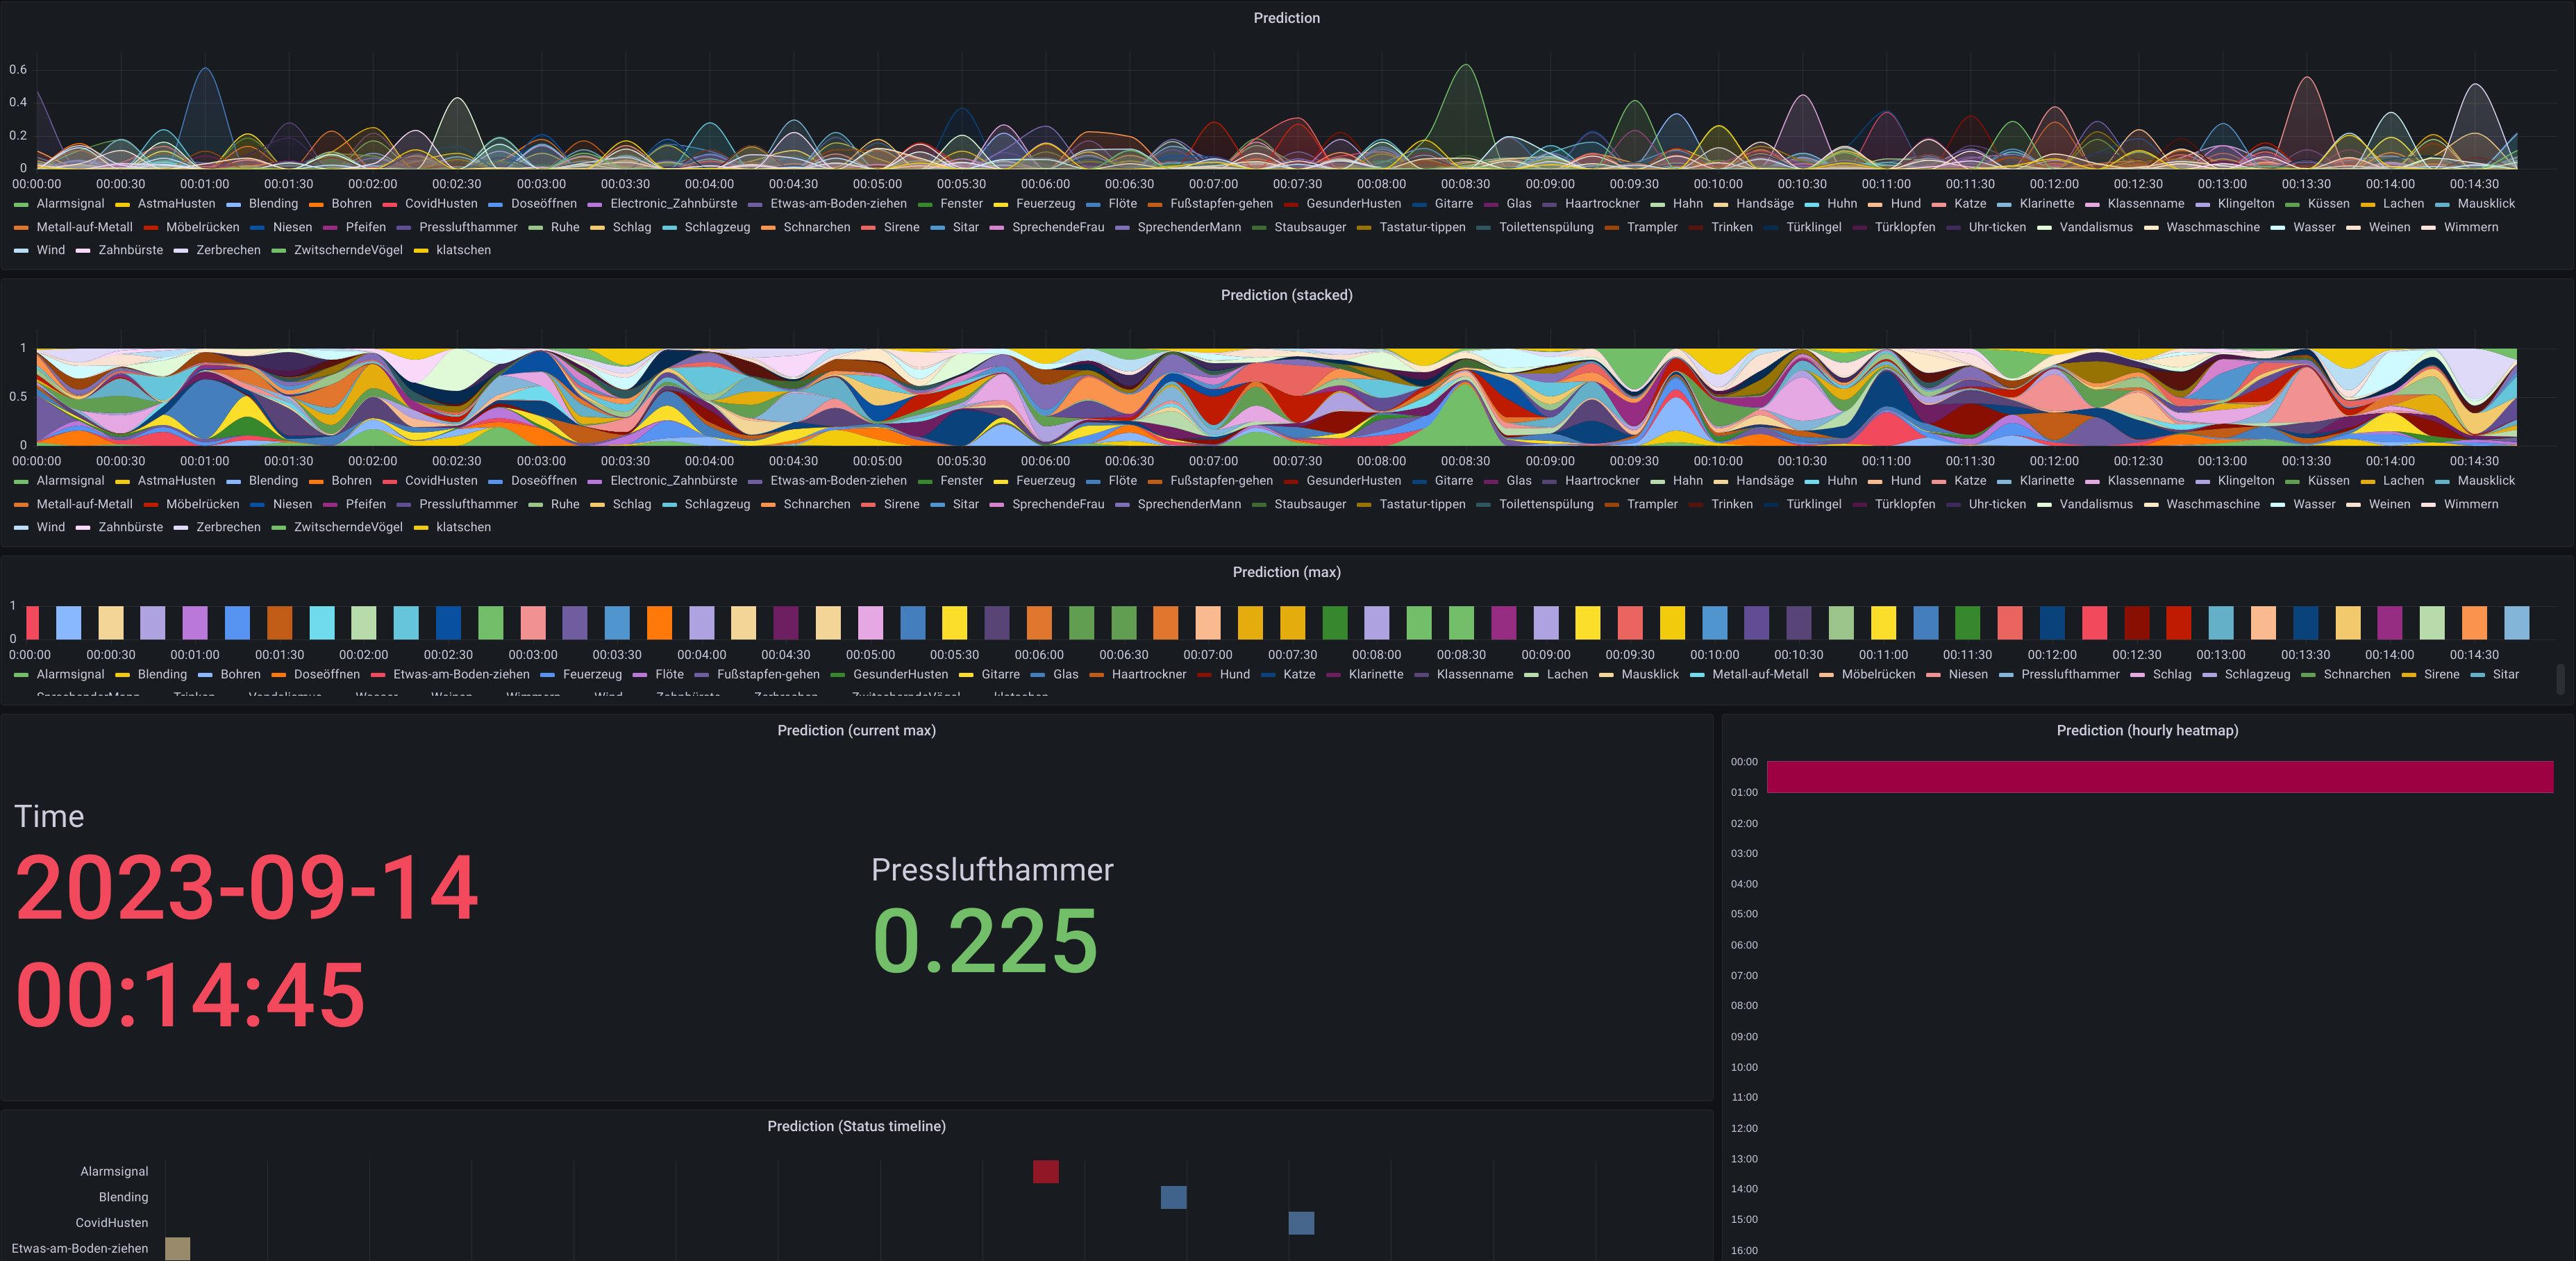
\includegraphics[width=0.85\textwidth]{Pictures/grafana}
  \caption{\label{fig:grafana}Grafana Dashboards}
\end{figure}

\subsubsection{\textsc{Alertmanager} Configuration}
% Setup and configuration of email alerts.
\textsc{Alertmanager} is integrated to handle alerts generated by \textsc{Prometheus}. A robust email notification system is set up, allowing for immediate alerting on predefined conditions.

\subsubsection{\textsc{Nginx} HTTP Server}
% Utilization of Nginx for serving static frontend builds.
\textsc{Nginx} is deployed to serve static frontend builds, ensuring fast and secure delivery of our frontend assets.

\subsubsection{\textsc{Traefik} Proxy}
% Configuration of Traefik proxy for domain name management and CSRF prevention.
\textsc{Traefik} is configured to enable the use of a single domain name for different services (frontend, backend API, MQTT), addressing same-origin requests problem. Integrated with \textsc{Cloudflare} and \textsc{LetsEncrypt}, \textsc{Traefik} also provides HTTPS support, enhancing the security of the system.

The overall Infrastructure is shown in \ref{fig:infra}.

\begin{figure}[htbp]
  \centering
  \begin{tikzpicture}[node distance=1cm, thick,
      block/.style={rectangle, draw, text width=6em, text centered, minimum height=4em}]

    % Nodes
    \node[block] (traefik) {Traefik};
    \node[block, below=of traefik] (nginx) {Nginx};
    \node[block, left=of nginx] (nodejs) {Node.js Backend};
    \node[block, right=of nginx] (mosquitto) {Mosquitto MQTT Broker};
    \node[block, right=of mosquitto] (mqttexporter) {MQTT-Exporter};
    \node[block, below=of mosquitto] (prometheus) {Prometheus};
    \node[block, below=of prometheus] (grafana) {Grafana};
    \node[block, above=of mqttexporter] (classifier) {Acoustic Event Classifier};

    % Connections
    \draw[->] (traefik) -- (nginx);
    \draw[->] (traefik) -- (nodejs);
    \draw[->] (traefik) -- (mosquitto);
    \draw[->] (nodejs) -- (prometheus);
    \draw[->] (mosquitto) -- (mqttexporter);
    \draw[->] (mqttexporter) -- (prometheus);
    \draw[->] (prometheus) -- (grafana);
    \draw[->] (classifier) -- (mosquitto);

  \end{tikzpicture}
  \caption{\label{fig:infra}Infrastructure}
\end{figure}

\subsection{Frontend Development}
\subsubsection{Framework and Styling}
% Choice of ReactJS and React-Router for the frontend framework.
% Use of Bootstrap v5 for styling and accessibility considerations.
% Application of D3.js for data visualization.

We choose \textsc{React.js} for its efficiency in rendering and updating components dynamically, essential for handling live data streaming. \textsc{react-router} is integrated using the \texttt{\lstinline{BrowserRouter}} for its compatibility and ease of creating a navigable single-page application. This approach allows us to create a seamless user experience without full page reloads. Routes are meticulously designed to facilitate easy navigation and logical access to different functionalities of the application. The structure of these routes includes:

\begin{itemize}
  \item \texttt{\lstinline{/live}} and \texttt{\lstinline{/live/:deviceId}} for accessing live data streams.
  \item \texttt{\lstinline{/device}} and \texttt{\lstinline{/device/:deviceId}} for device management.
  \item \texttt{\lstinline{/alert}} and \texttt{\lstinline{/alert/:alertId}} for alert management.
  \item \texttt{\lstinline{/query}} and \texttt{\lstinline{/query/:visualizationType}} for querying and visualizing historical data.
  \item \texttt{\lstinline{/settings}} for configuration settings.
  \item \texttt{\lstinline{/logout}} for user logout functionality.
\end{itemize}

We select Bootstrap v5 as our basic design system. It provides a robust foundation for styling basic elements and we use it to ensure a responsive layout across various devices and screen sizes. We leverage Bootstrap's grid system to establish the basic layout of the application, ensuring that each component and page is both aesthetically pleasing and functional. We give special attention to making the interface accessible, aligning with Bootstrap’s accessibility features.

For the data visualization aspect of our frontend, we choose \textsc{D3.js} library to create complex and interactive visualizations, which is a core requirement for representing the classifier’s real-time data. We utilize \textsc{D3.js} to implement a dynamic heatmap visualization, which presents the classification results in an understandable and insightful manner.

The integration of D3.js with \textsc{React.js} posed certain challenges due to their differing approaches to DOM manipulation. To overcome this, we develop custom hooks in \textsc{React.js} to encapsulate \textsc{D3.js} code, ensuring that the \textsc{D3.js} visualizations were seamlessly integrated into the \textsc{React.js} component lifecycle. This approach maintains \textsc{React.js}'s declarative nature while leveraging \textsc{D3.js}'s powerful data-driven transformation capabilities.

\subsubsection{Single Page Web Application Development}
% Development process of the single-page application.
% Integration with the MQTT server for live data streaming.

We utilize \textsc{mqtt.js} to establish a reliable connection for live data streaming from the acoustic event classifier. This allows for the real-time reception of data on the frontend. \textsc{D3.js} is employed to render this data stream into an intuitive and interactive heatmap. The visualization represents the last 60 seconds of data on the x-axis, with classification tags on the y-axis. The color intensity in the heatmap corresponds to the confidence level of each prediction. We face challenges in synchronizing the high-velocity data stream with the \textsc{D3.js} visualization. To address this, we implement efficient data-binding techniques and optimize the rendering process to ensure smooth, real-time updates.

We developed calendar heatmap components by embedding \textsc{Grafana} visualization plugins. This allows us to present historical data in a calendar format, providing users with an easy way to navigate and analyze past events. Special attention is paid to making this component user-friendly and visually appealing. We ensure that it is seamlessly integrated with the overall design of the web application.

User settings and preferences were stored in LocalStorage. This choice provided a simple and effective way to persist user-specific settings without the need for backend storage solutions.

We integrate \textsc{web-vitals} to collect key metrics like Cumulative Layout Shift (CLS), First Input Delay (FID), First Contentful Paint (FCP), Largest Contentful Paint (LCP), and Time to First Byte (TTFB). These metrics guide our optimization efforts during development. We use \textsc{stat.js} to display real-time performance metrics such as frames per second (FPS) and memory usage to users. This feature is particularly useful for monitoring the application's responsiveness and resource consumption.

To enhance user interaction, we implement a notification center using \textsc{react-toastify}. This allows us to display alerts and messages to users in a non-intrusive and user-friendly manner. The design and placement of notifications are carefully considered to ensure they are informative yet unobtrusive, enhancing the overall user experience.

\subsection{Technical Challenges and Solutions}
In this section, we will highlight some of the significant technical challenges encountered during the development of the acoustic event classification demonstration and the strategies employed to overcome these obstacles. This section aims to provide insights into problem-solving approaches and the application of technical knowledge in practical scenarios.


\subsubsection{Frontend Performance Optimization}
% Techniques used to optimize the performance of the system.
The core functionality of the system involves real-time processing and visualization of acoustic event classification data. This requires the system to handle continuous data streams efficiently and render visualizations with minimal latency. The challenge is to ensure that the live data stream from the MQTT server is processed and displayed in a heatmap format without significant delays, ensuring a seamless user experience.

To address this, \textsc{D3.js} transitions are used for dynamic data visualization. The rendering of each piece of data is called only once and the elements will be removed when they are outside the viewport of the visualization. This is to minimize unnecessary re-rendering, thus enhancing performance. With hooks of \textsc{React.js}, the side effects are well managed, and cleanups are done when the heatmap component is unmounted.

\subsubsection{User-Friendly and Accessible Design}
The system needs to be not only technically sound but also user-friendly and accessible to a diverse range of users. The challenge is to create an intuitive interface that caters to both technical and non-technical users.

User experience (UX) principles are carefully considered during the design phase. This involved creating intuitive navigation and clear, understandable visualizations. Bootstrap v5 is utilized for responsive design, ensuring that the application is accessible on various devices and screen sizes.
Feedback from initial user testing is incorporated to refine the UI/UX, ensuring that the system is easy to use and meets the needs of its users.

\subsubsection{Security Considerations}
% Security measures implemented throughout the development process.
With the system handling sensitive data and being accessible over the internet, ensuring security and data privacy is paramount. This includes protecting against common web vulnerabilities and securing data transmission.

Security measures such as HTTPS support with Cloudflare and Let's Encrypt are carried out to encrypt data in transit. \textsc{Mosquitto’s} file-based user and ACL management are used to control access and ensure that users can access only what they are authorized to. Regular security audits are conducted, and industry-standard security practices like OWASP Application Security Verification Standard (ASVS) are followed to protect against common web vulnerabilities like CSRF, XSS, and SQL injection.

\subsection{Project Management and Development Practices}
% If applicable, detail the use of Agile methodologies in project management.
% Utilization of version control systems and collaborative tools.
In the development of the acoustic event classification demonstration, project management and development practices are carried out to ensure an organized and efficient workflow. Central to these practices is the use of GitHub for issue tracking and version control.

\subsubsection{Issue Tracking with GitHub}
The project leveraged GitHub's issue-tracking system to organize tasks, bugs, and feature requests. Each issue is clearly defined with labels for easy categorization and prioritization. Milestones are created on GitHub to group issues into manageable phases, aligning with specific development goals and timelines. This helps in maintaining a clear vision of the project roadmap and deadlines. The progress of each issue is regularly updated, providing transparency and allowing for real-time tracking of the project's advancement.

\subsubsection{Version Control and Collaboration}
A structured branching strategy is employed, with separate branches for features, hotfixes, and releases. This approach ensures that the development of new features does not disrupt the main codebase. Automated build and test processes are integrated into the GitHub repository, ensuring that each commit and merge request adheres to the project's quality standards.
\chapter{Results}
% - Present the newly designed web-based acoustic event classification model.

\section{Demonstration of the Web-Based Model}
% - Discuss how the redesign enhances user-friendliness and accessibility.
% - Include user feedback or case studies.


\subsection{System Architecture and Implementation}
% - Detailed walkthrough of the backend and frontend setup
% - Explanation of the docker compose environment, Eclipse Mosquitto, Prometheus, Grafana, Alertmanager, Nginx, and Traefix proxy
% - Description of the MQTT-exporter and its integration with Prometheus
This section provides a comprehensive demonstration of the our web-based result, focusing on both the backend and frontend implementations, as well as the setup of the supporting infrastructure.

\subsubsection{Backend Architecture}
The core of the system is a robust backend server responsible for device management, alert management, and providing an API for reloading \textsc{Prometheus} alert rules. The MQTT-exporter, designed to record classifier results and expose them to \textsc{Prometheus} in a format compatible with \textsc{Prometheus} runs sound and safe.

\begin{figure}[htbp]
  \centering
  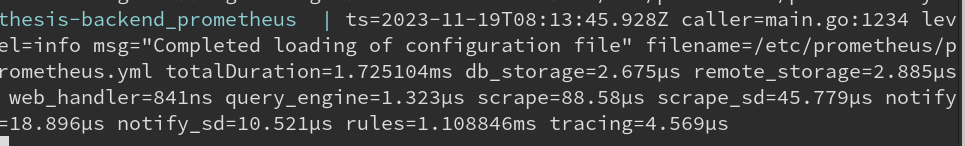
\includegraphics[width=0.85\textwidth]{Pictures/prometheusreload}
  \caption{\label{fig:prometheusreload}\textsc{Prometheus} successfully reload when the API is called properly}
\end{figure}

\subsubsection{Infrastructure Setup}
The system operates within a \textsc{Docker Compose} environment, in an isolated network namespace, ensuring security, scalability and ease of deployment. The services running includes our backend APIs, \textsc{Eclipse Mosquitto} with file-based user and access control list (ACL) management, \textsc{Prometheus}, \textsc{Grafana} and \textsc{mosquitto-exporter} exposing metrics to \textsc{Prometheus} for comprehensive monitoring.

\begin{figure}[htbp]
  \centering
  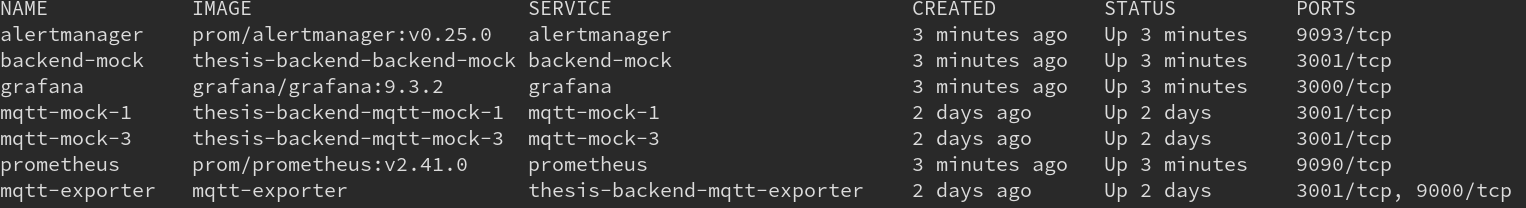
\includegraphics[width=0.85\textwidth]{Pictures/dockerps}
  \caption{\label{fig:dockerps}Running \textsc{Docker} Services}
\end{figure}

\subsubsection{Frontend Interface}
The frontend is deployed statically and is served by \textsc{Nginx}. \textsc{Bootstrap v5} is employed for styling, emphasizing accessibility and a user-friendly interface. The application showcases a single-page layout for streamlined user interaction. Additionally, intuitive interfaces are provided for managing devices and alerts.

\begin{figure}[htbp]
  \centering
  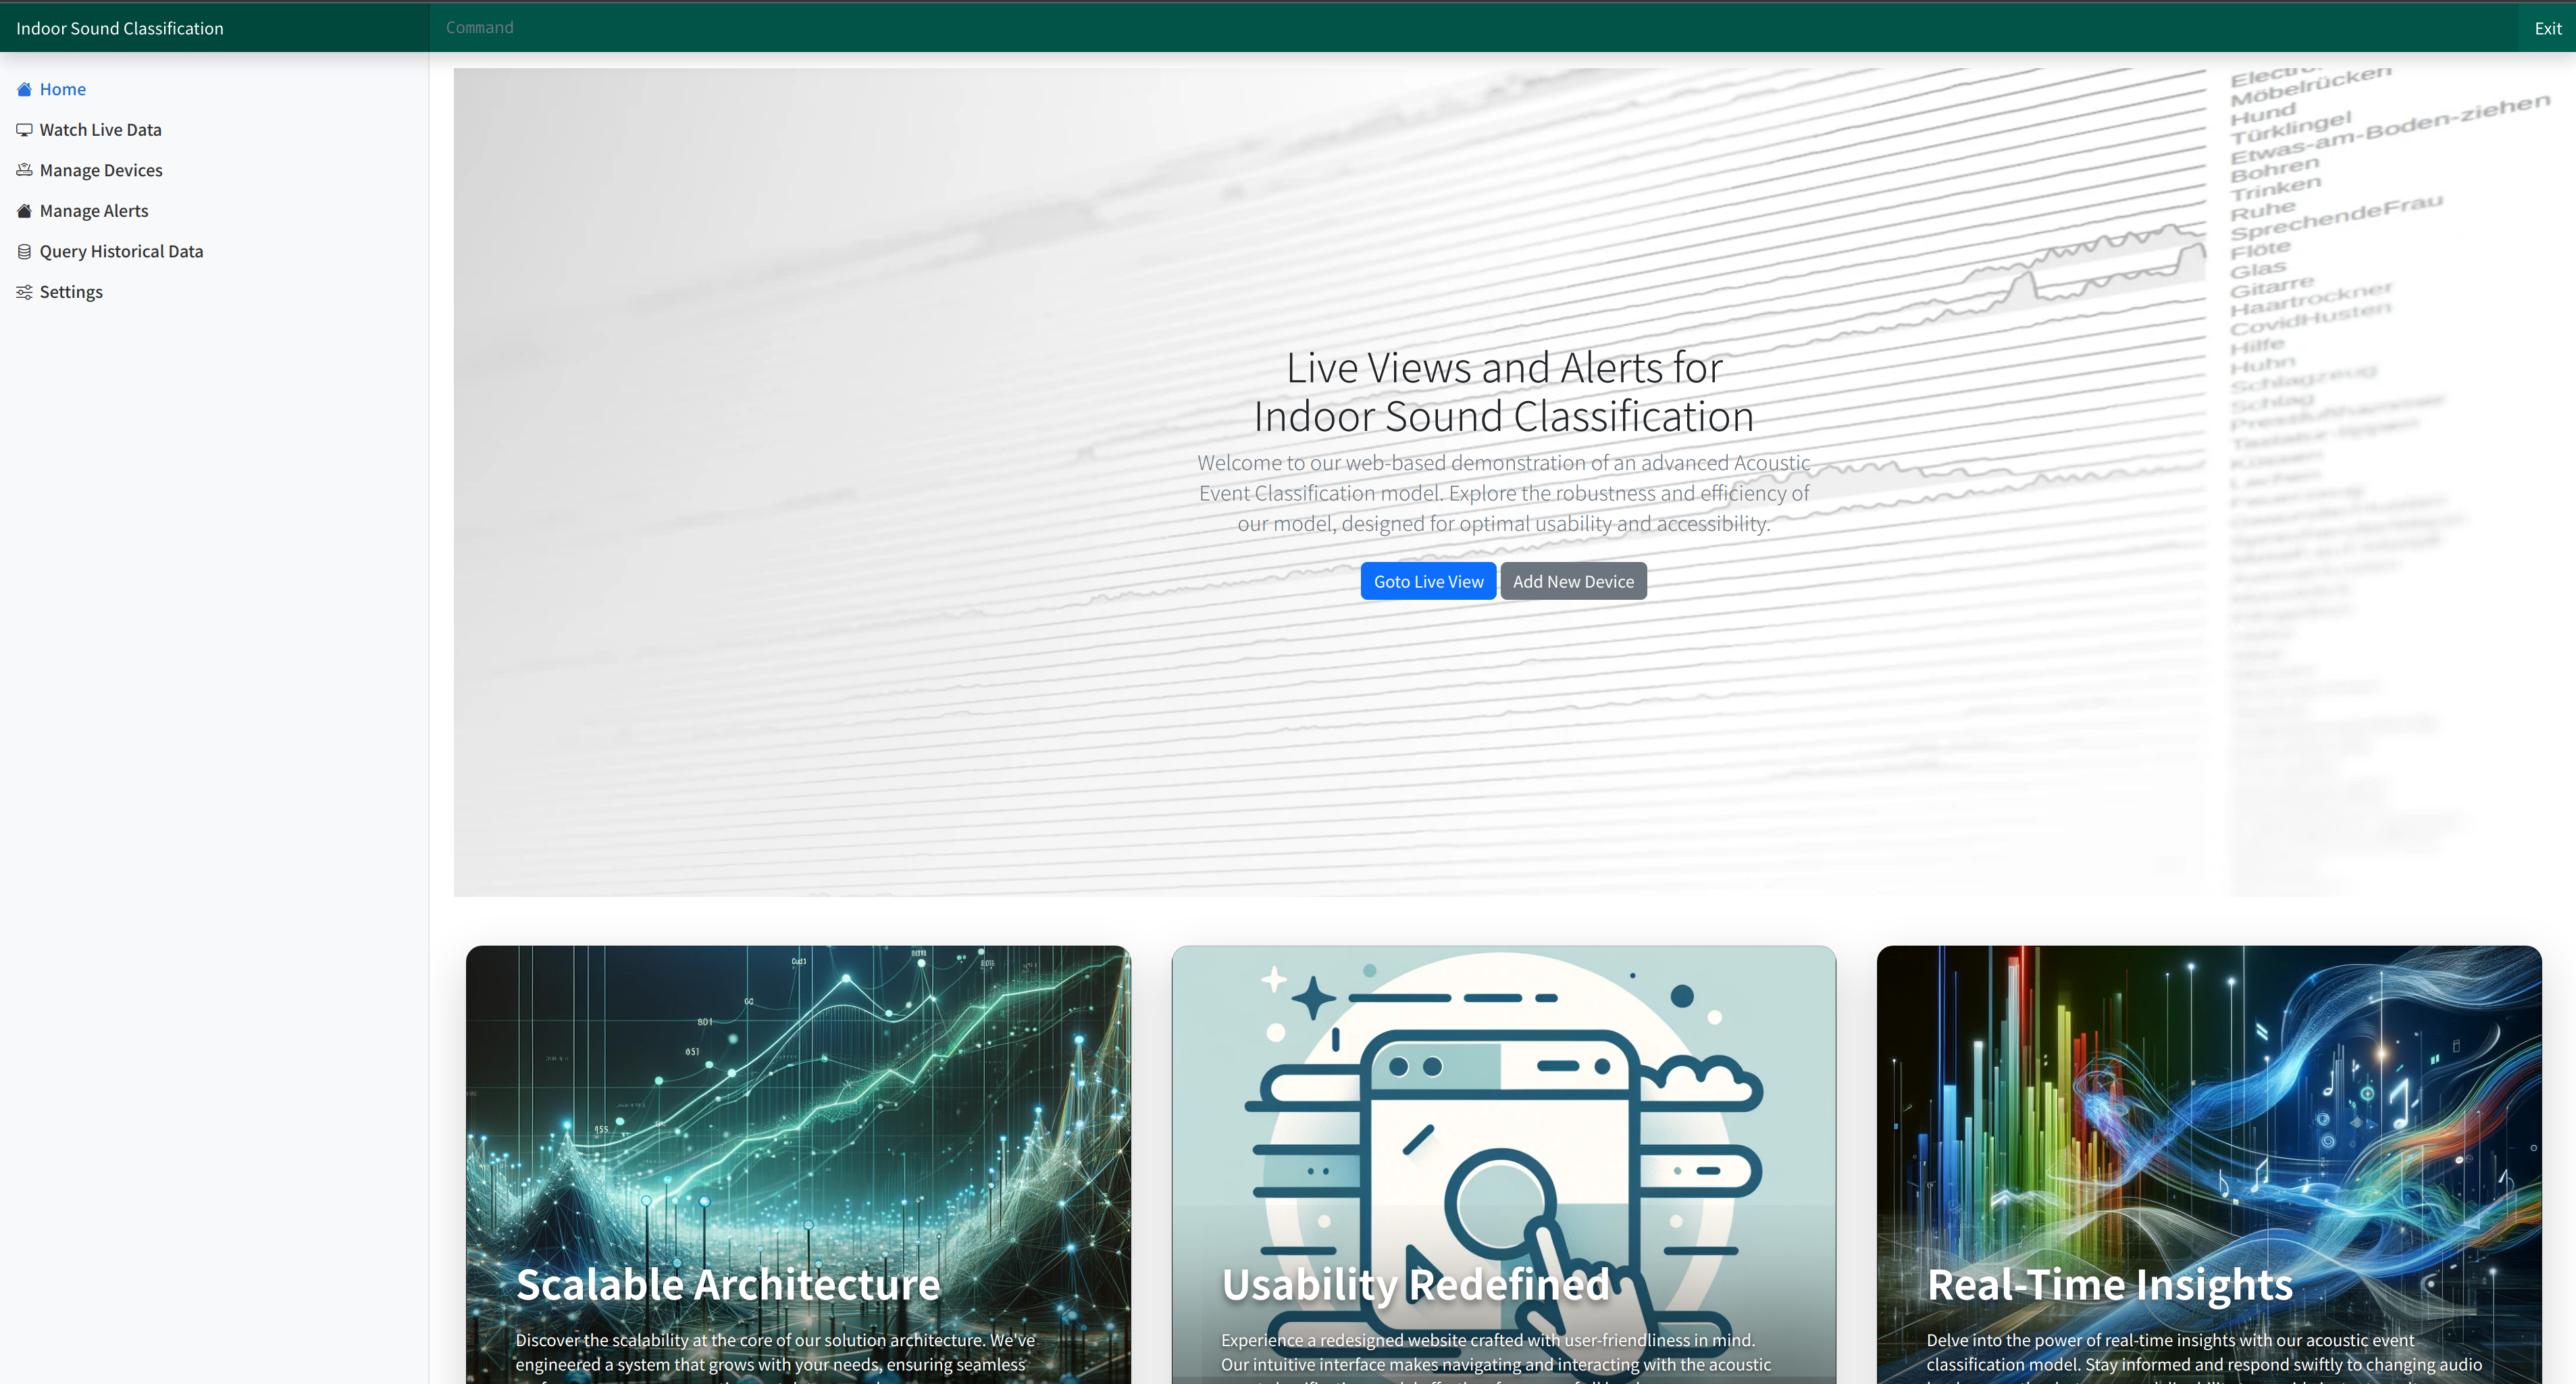
\includegraphics[width=0.85\textwidth]{Pictures/home}
  \caption{\label{fig:schome}Landing Page Design}
\end{figure}

\subsubsection{Data Visualization and Management Interfaces}
The live view feature subscribes to the MQTT server, presenting a real-time data stream from the acoustic event classifier. This data is rendered in a heatmap format, with the last 60 seconds on the X-axis and classification tags on the Y-axis. The color intensity represents the confidence level of predictions.

% Insert Screenshot: Live View and Heatmap Visualization]


\subsection{Frontend Interface and Features}
% - Overview of the single-page web application built with ReactJS
% - Description of key features:
%   - Live view subscribing to MQTT server
%   - Heatmap visualization of real-time data
%   - Interfaces for classifier and alert management
%   - Historical data visualization and server credential settings

\subsubsection{Single Page Web Application}
A streamlined, single-page application allows for real-time monitoring and management without the need for reloading or navigating multiple pages.

\subsubsection{Heatmap Visualization}
The innovative heatmap visualization offers a quick and intuitive understanding of the classifier's real-time output. The visualization uses time (last 60 seconds) as the X-axis and classification tags as the Y-axis, with varying color intensities indicating prediction confidence.

\begin{figure}[htbp]
  \centering
  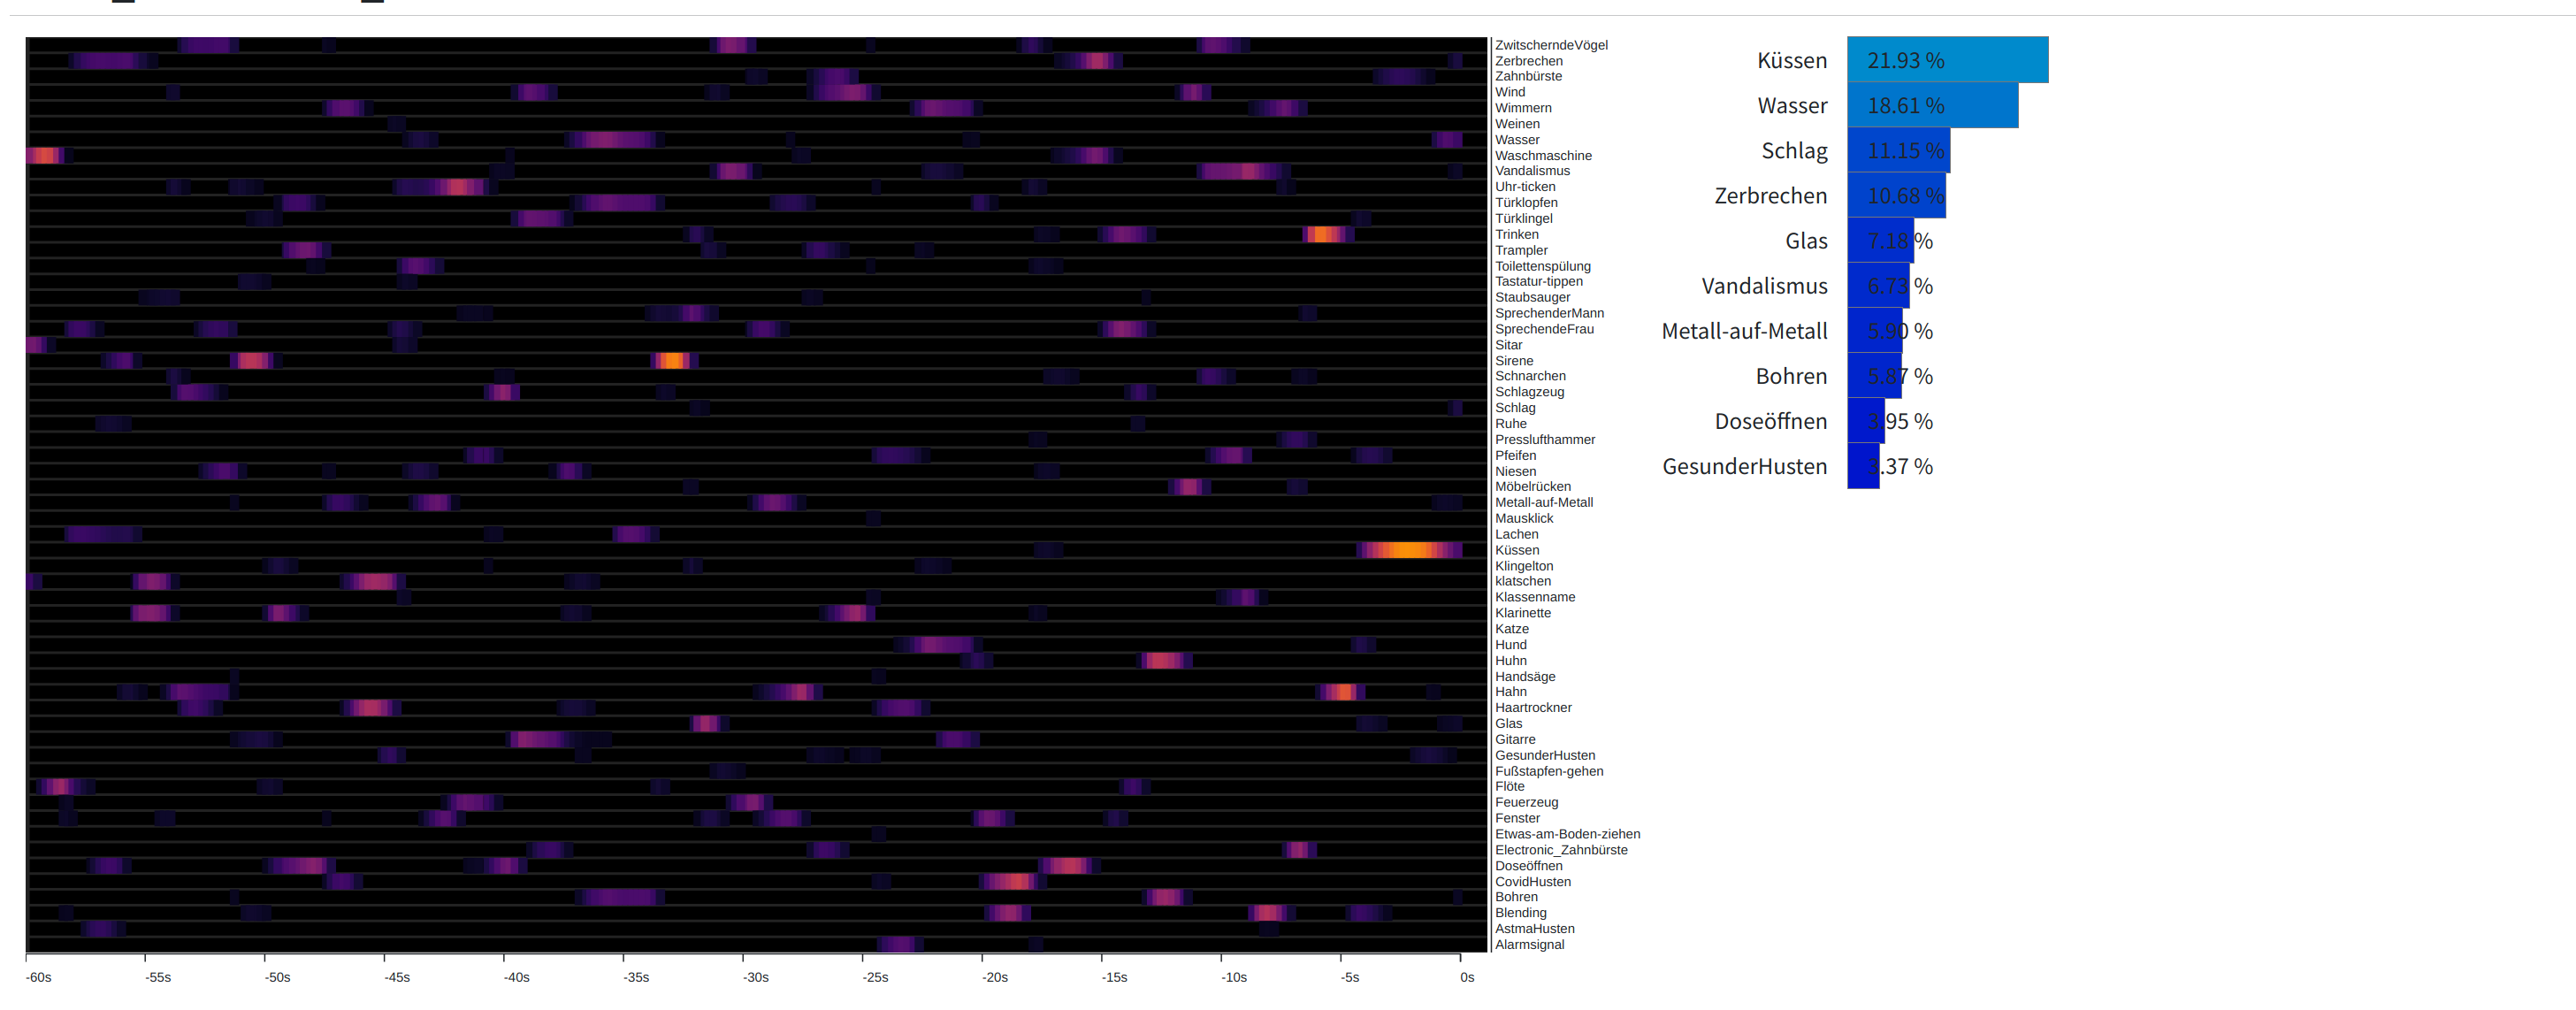
\includegraphics[width=0.85\textwidth]{Pictures/heatmap}
  \caption{\label{fig:heatmap}Live Streaming Data Visualization}
\end{figure}

\subsubsection{Classifier and Alert Management}
The interfaces for managing classifiers and alerts are designed for ease of use, allowing users to seamlessly control and configure the system according to their specific needs.

\begin{figure}[htbp]
  \centering
  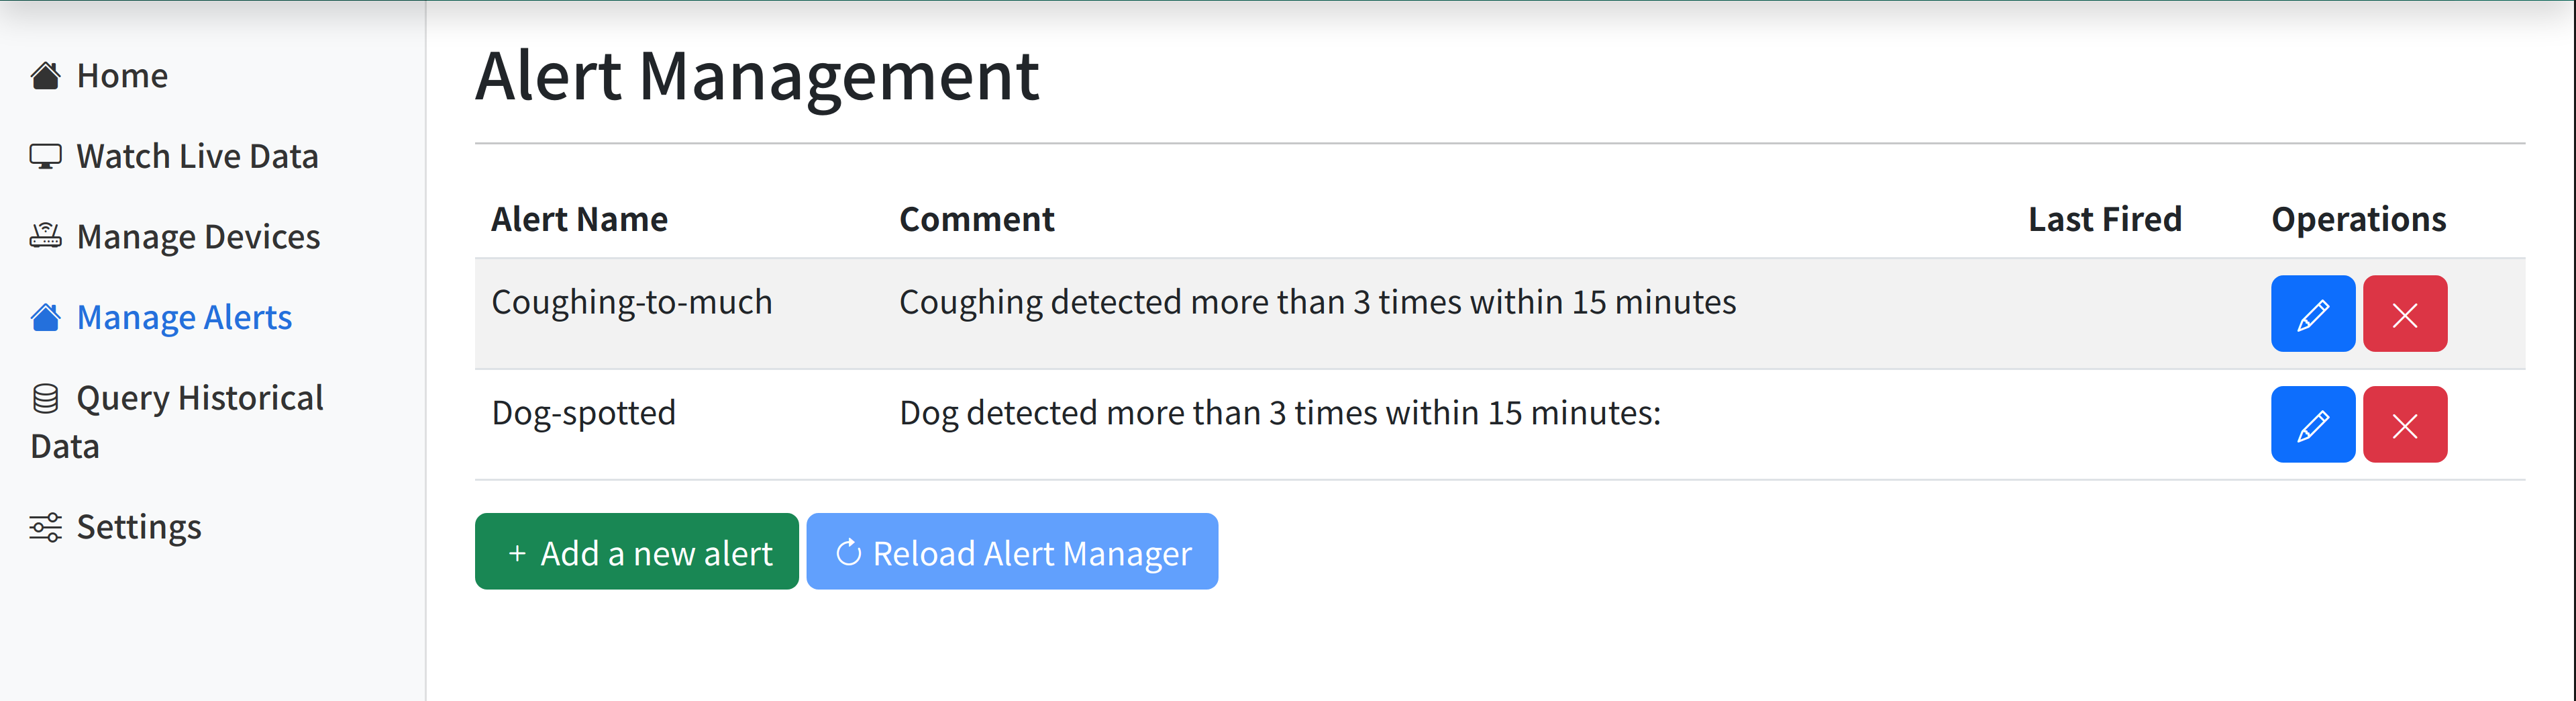
\includegraphics[width=0.85\textwidth]{Pictures/alertmanagement}
  \caption{\label{fig:alertmanagement}Alert Management Interface}
\end{figure}

\begin{figure}[htbp]
  \centering
  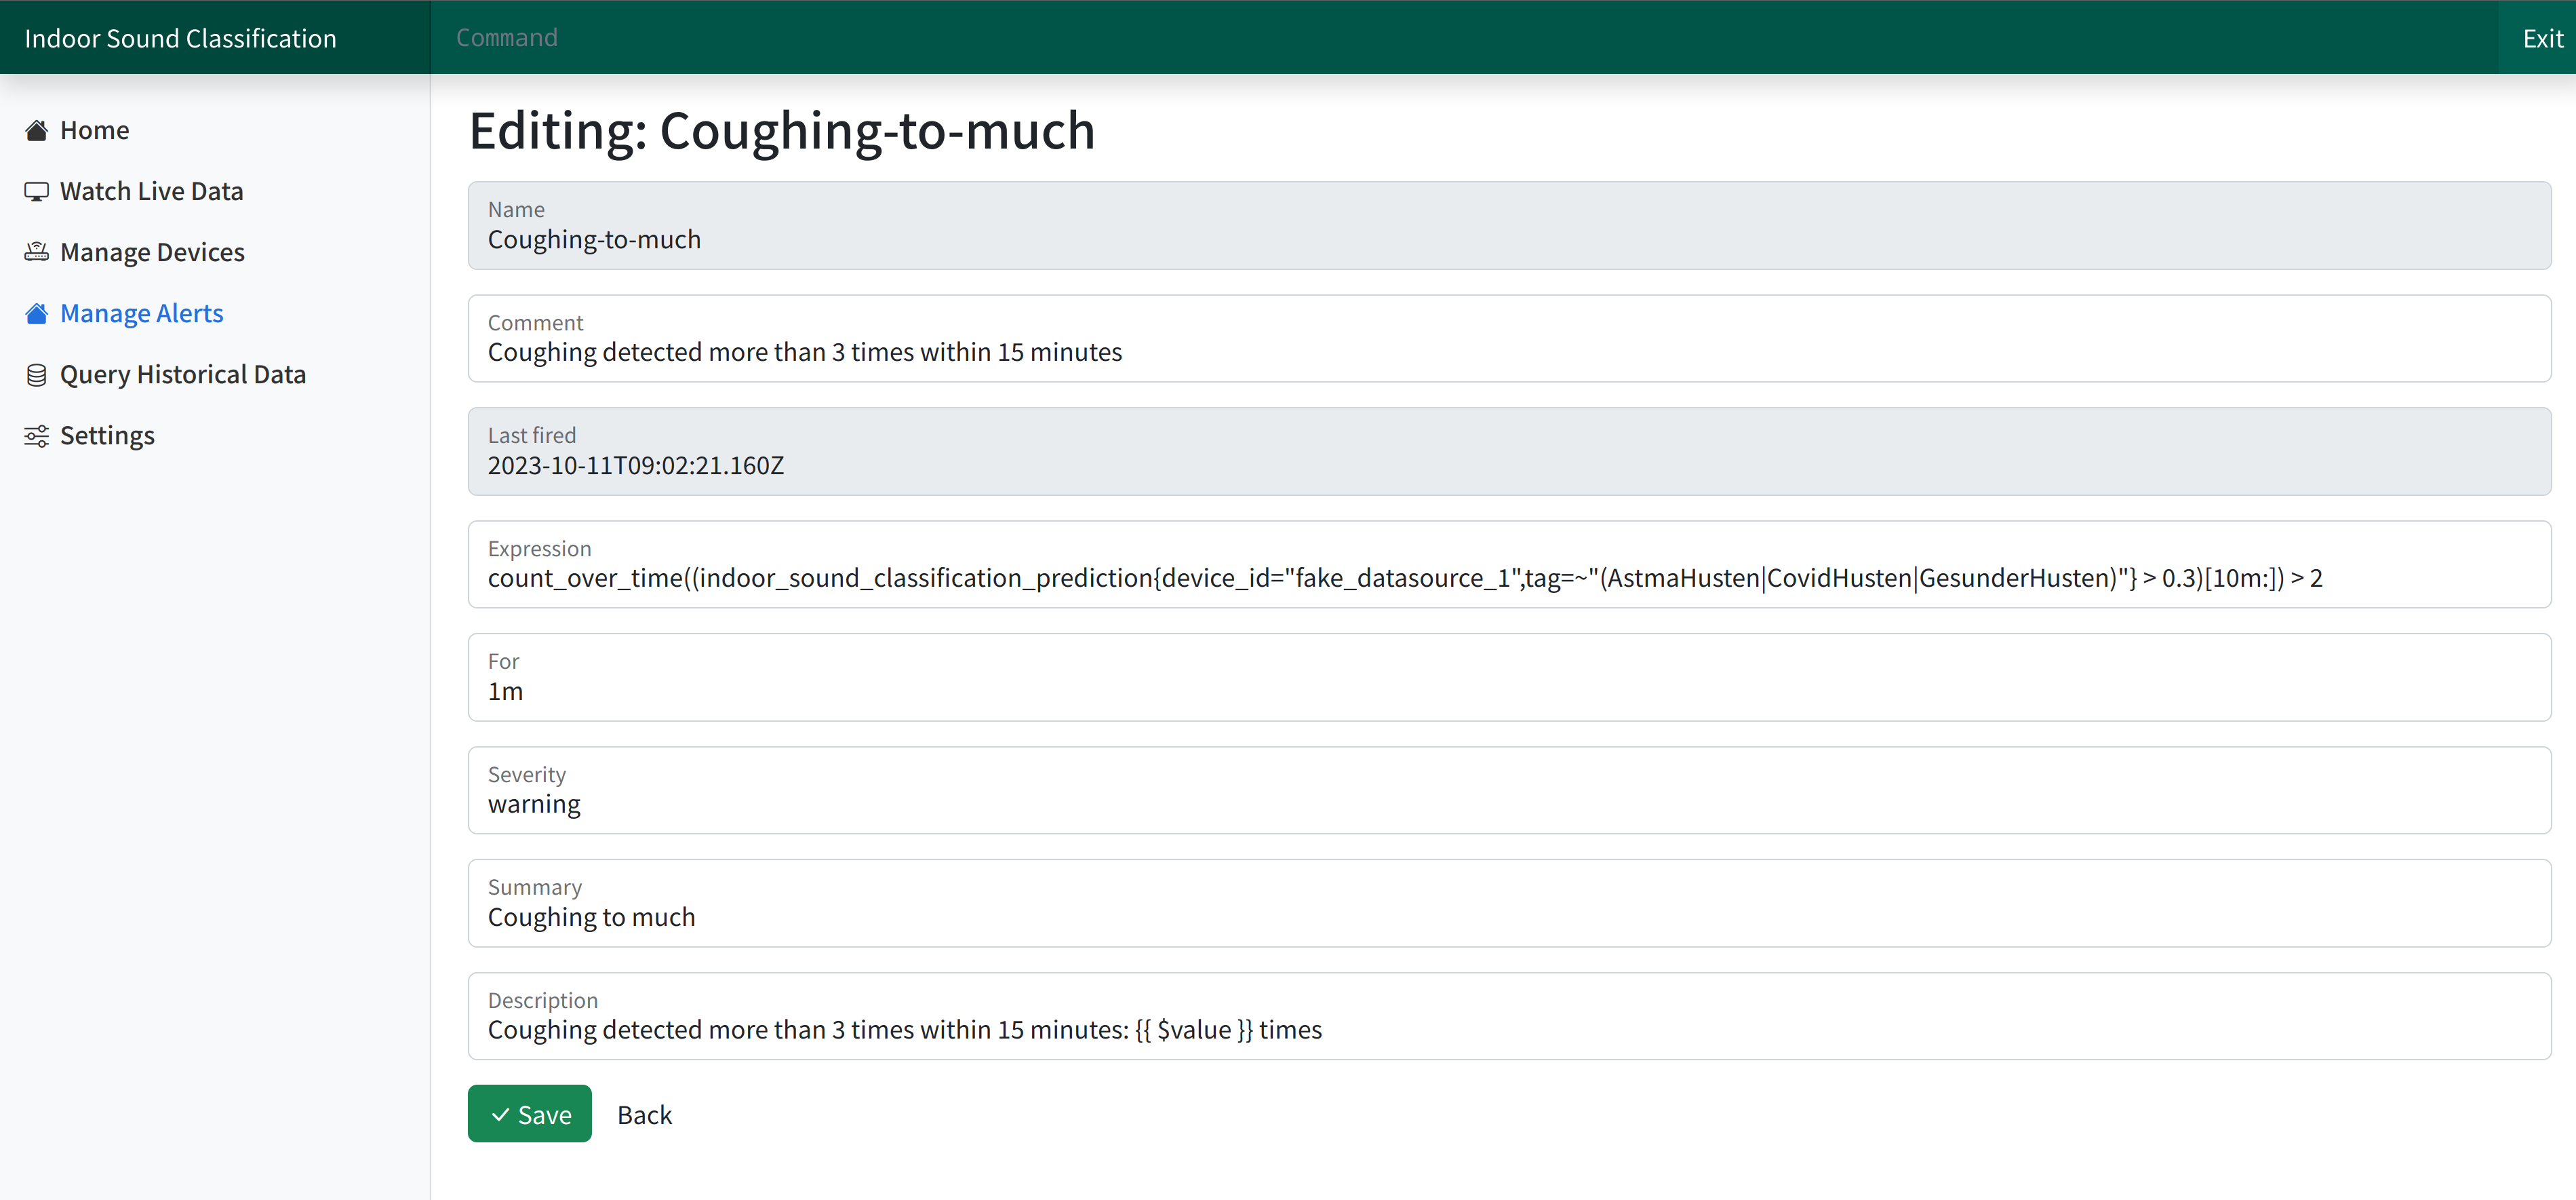
\includegraphics[width=0.85\textwidth]{Pictures/alertedit}
  \caption{\label{fig:alertedit}Alert Editing Interface}
\end{figure}

\subsubsection{Settings and Configuration}: A dedicated settings page is included for users to easily input and update server credentials, ensuring secure and personalized access to the system.

\subsubsection{Historical Data Visualization}
The application also provides various visualizations of historical data, extracted from \textsc{Prometheus} TSDB via \textsc{Grafana}, aiding in long-term analysis and trends observation.

\begin{figure}[htbp]
  \centering
  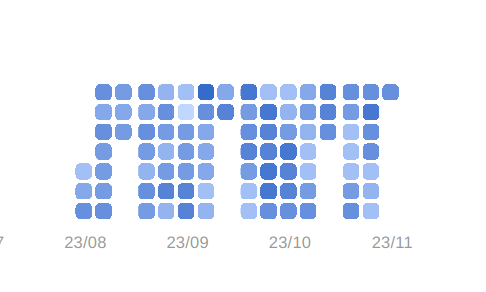
\includegraphics[width=0.85\textwidth]{Pictures/calendar-weekday-day}
  \caption{\label{fig:calendar-weekday-day}Calendar View of Event Frequencies}
\end{figure}
\subsubsection{Settings and Configuration}: A dedicated settings page is included for users to easily input and update server credentials, ensuring secure and personalized access to the system.

\begin{figure}[htbp]
  \centering
  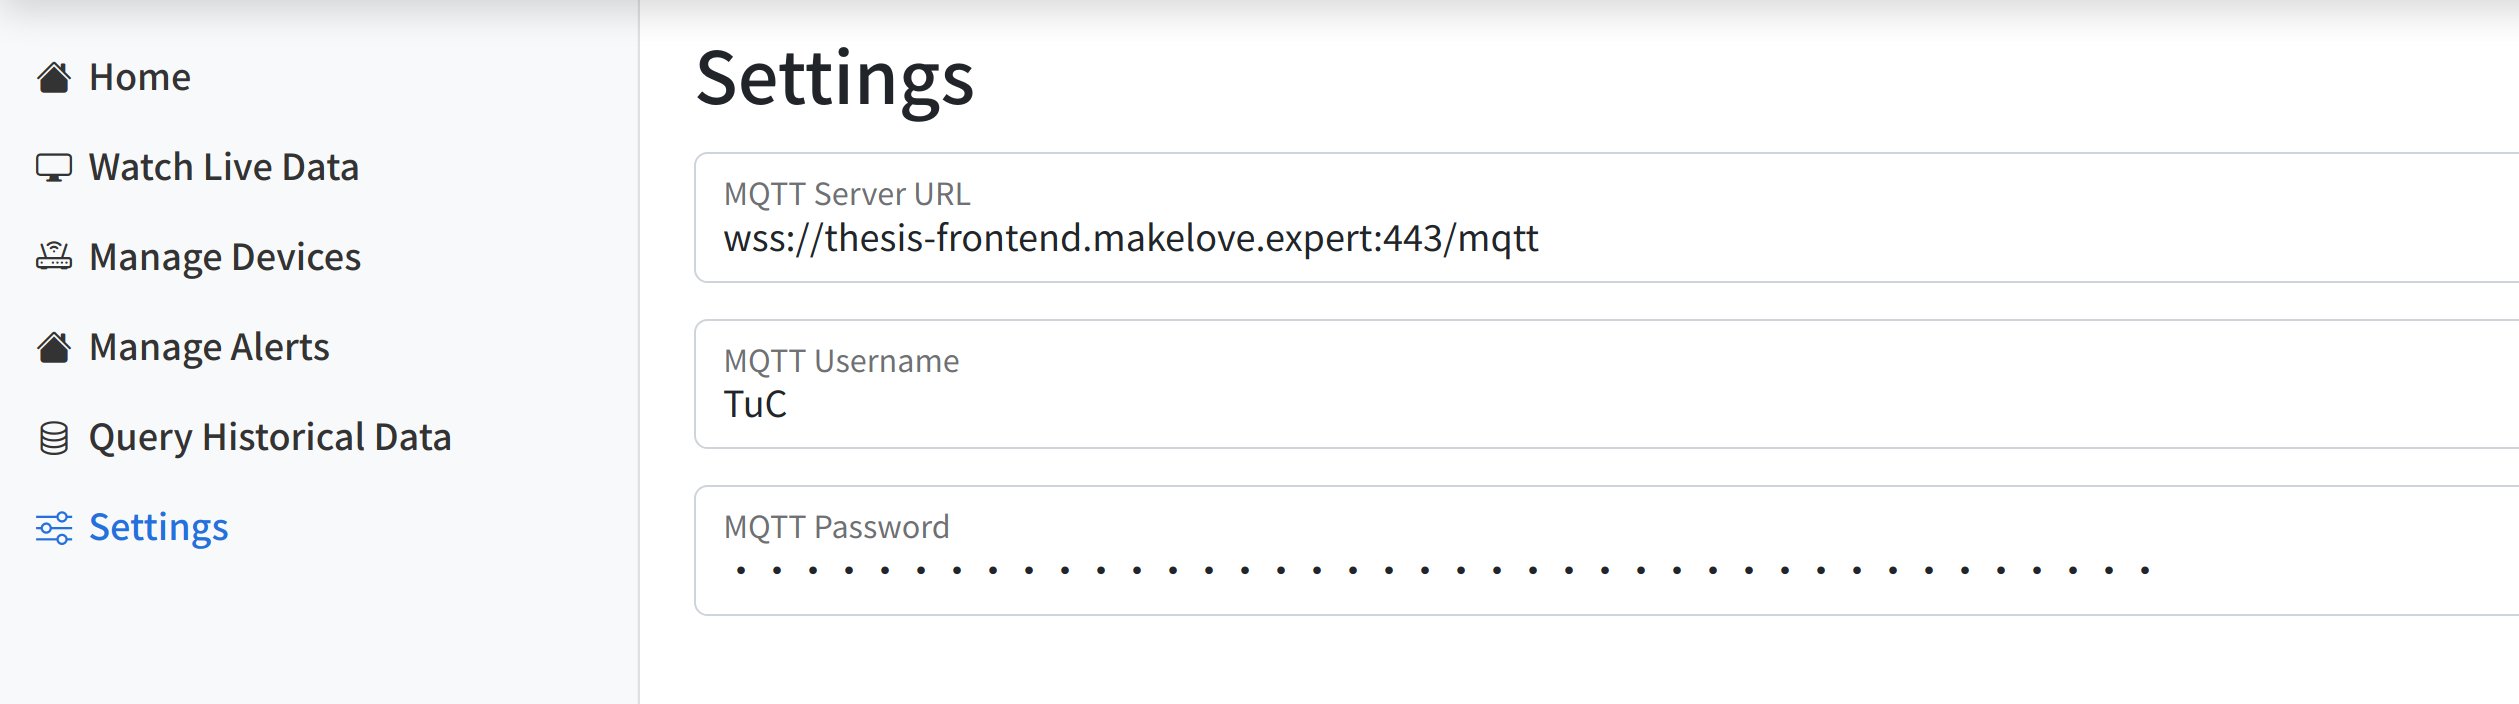
\includegraphics[width=0.85\textwidth]{Pictures/settings}
  \caption{\label{fig:settings}Settings Interface}
\end{figure}


In summary, the web-based model demonstrates a cohesive integration of backend robustness with frontend accessibility, underpinned by a user-friendly interface and effective data visualization techniques. The system architecture not only addresses the technical requirements of acoustic event classification but also emphasizes the importance of user experience and accessibility.

\section{Testing of the Alert System}
% - Simulation tests to assess the effectiveness of the alert system, including the responsiveness and accuracy of email alerts.
% - Performance analysis of the alert manager in various simulated emergency scenarios.
\subsection{Test Setup and Methodology}
In order to evaluate the effectiveness and reliability of the alert system, a comprehensive testing strategy is implemented. The test environment is configured to mimic real-world conditions as closely as possible. This involves setting up the complete system architecture, including the backend server, MQTT-exporter, and the integration with \textsc{Prometheus} and \textsc{Alertmanager}.

The methodology involves generating a series of simulated acoustic events, which were then classified and processed by the system. These events were designed to test the system's ability to accurately detect and categorize different types of acoustic signals, and subsequently trigger appropriate alerts.

We use perlin noise to simulate acoustic events. The predictions of the classifier are broadcasted by \textsc{Mosquitto} and the MQTT-exporter records the result. \textsc{Prometheus} scrapes the result from MQTT-exporter and evaluate the alert rules, and in the end trigger the \textsc{Alertmanager} to send alerts by email.

\subsection{Test Results}
\subsubsection{Alert Triggering}
The tests showed that the alerts were successfully triggered under specific conditions designed to mimic real acoustic events. For instance, when a predefined sound pattern was detected, the system promptly identified it and triggered the corresponding alert. This demonstrates the system's ability to react accurately to environmental cues.

\subsubsection{Alert Rules Evaluation Time}

A critical aspect of the alert system's performance is the speed of alert rule evaluation. During testing, the average alert rules evaluation time was measured to be approximately 145 milliseconds. This quick response time is essential in situations where timely alerts are crucial, and it underscores the system's efficiency.

% screenshot alert rules evaluation time

\subsubsection{Email Notification Delivery}
The effectiveness of the alert system also depends on the successful delivery of notifications. In this regard, the system performed admirably. Emails generated as a result of the triggered alerts were sent and successfully delivered to the recipients' mailboxes. This was verified through a combination of automated scripts and manual checks. The emails contained detailed information about the alert, including the time of occurrence and the specific nature of the acoustic event.

\begin{figure}[htbp]
  \centering
  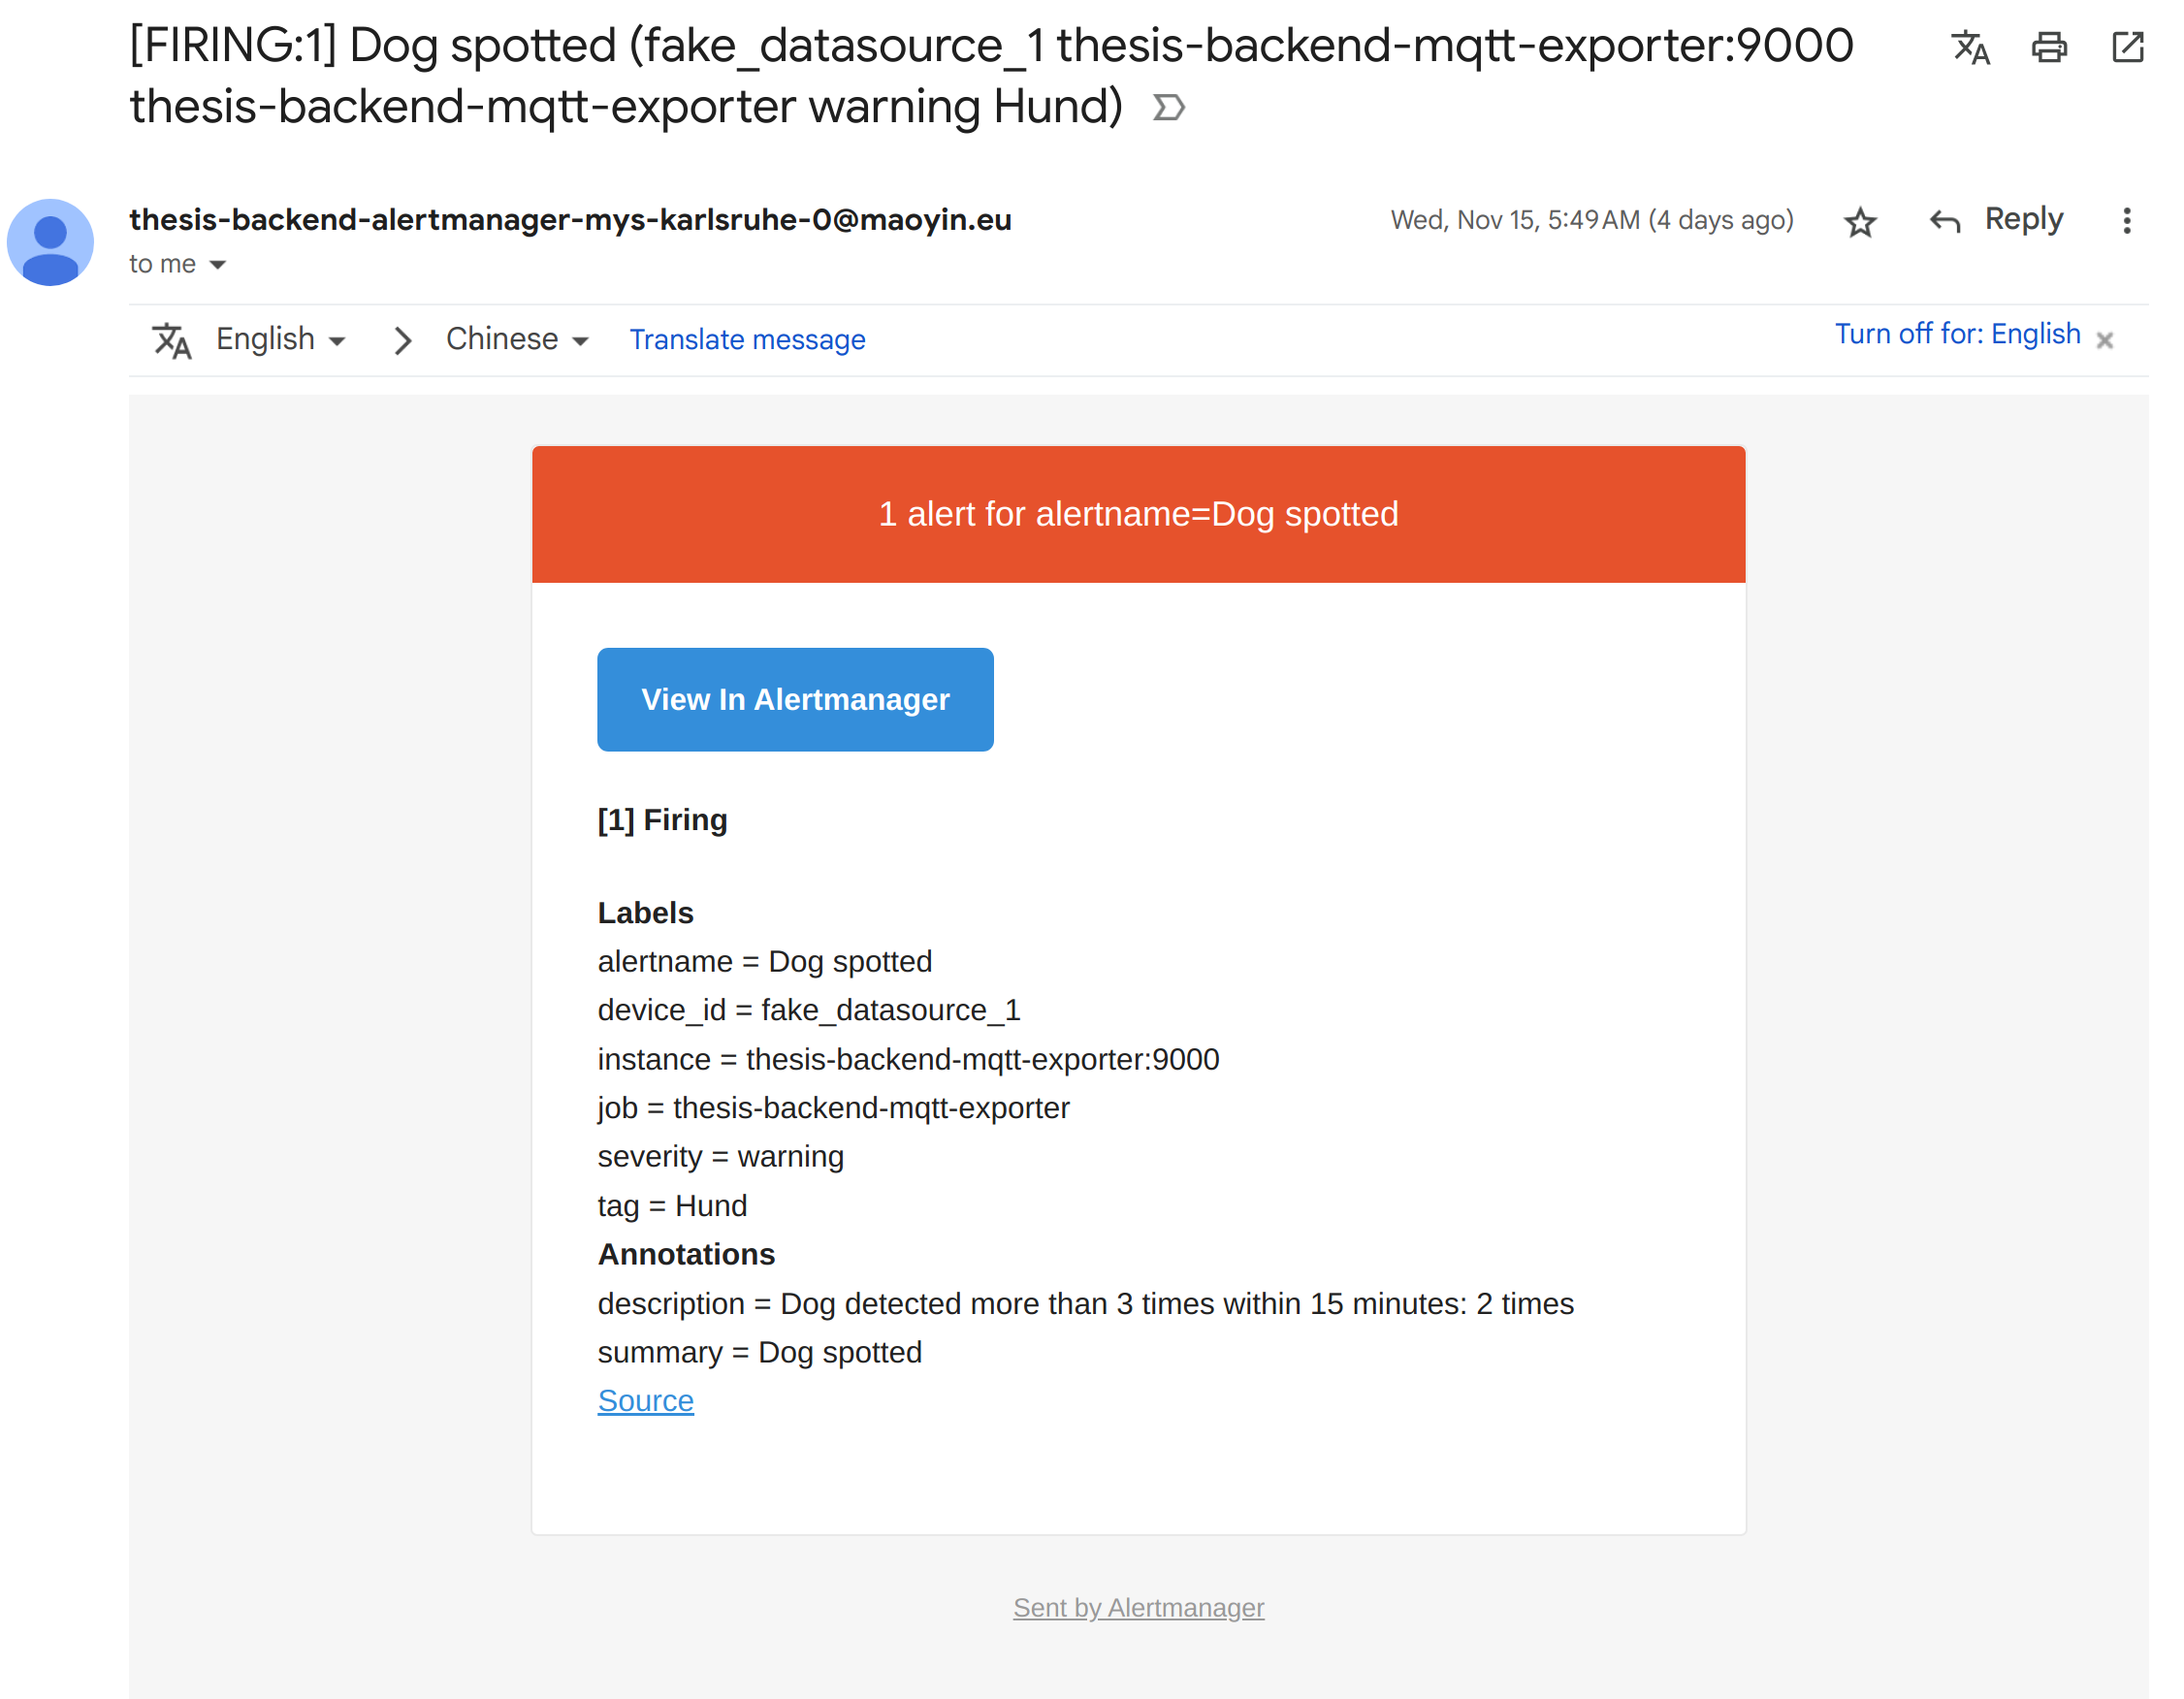
\includegraphics[width=0.85\textwidth]{Pictures/email}
  \caption{\label{fig:email}The Delivered Alert Email}
\end{figure}

The tests conducted on the alert system have conclusively demonstrated its reliability and efficiency. The system's ability to promptly trigger alerts, quickly evaluate alert rules, and effectively deliver email notifications, all within a fraction of a second, speaks to its robustness and practicality in real-world applications. These results are a testament to the successful implementation of the alert system within the broader framework of the acoustic event classification model.

\section{User-Friendliness and Accessibility}
% - Present the results of usability and accessibility testing.
% - Discuss how the web-based solution fulfills these aspects.
\subsubsection{Web Accessibility Evaluation}
The web application was rigorously evaluated for accessibility using a range of Web Accessibility Evaluation Tools. These tools assess key areas such as screen reader compatibility, keyboard navigation, and adherence to the Web Content Accessibility Guidelines (WCAG).

\subsubsection{Evaluation Results}
\begin{itemize}
  \item \textbf{Screen Reader Compatibility}: The application was tested with several leading screen readers. Results indicated high compatibility, with screen readers effectively interpreting and voicing out content and navigation elements.
  \item \textbf{Keyboard Navigation}: The application supports comprehensive keyboard navigation. Testing showed that users could navigate through all interactive elements using the keyboard, a vital feature for users with motor impairments or those who prefer keyboard inputs.
  \item \textbf{Screen Reader Compatibility}: The application was tested with several leading screen readers. Results indicated high compatibility, with screen readers effectively interpreting and voicing out content and navigation elements.
  \item \textbf{Keyboard Navigation}: The application supports comprehensive keyboard navigation. Testing showed that users could navigate through all interactive elements using the keyboard, a vital feature for users with motor impairments or those who prefer keyboard inputs.
  \item \textbf{Color Contrast and Text Readability}: The evaluation tools checked for color contrast ratios and text readability. The application meets the recommended contrast ratios, ensuring that text is legible and distinguishable for users with visual impairments.
  \item \textbf{ALT Tags and ARIA Labels}: The usage of ALT tags for images and ARIA labels for interactive elements was found to be consistent and descriptive, aiding users who rely on assistive technologies to understand and interact with the content.
  \item \textbf{Responsive Design}: The application's responsive design was tested across various devices and screen sizes. This ensures accessibility and usability irrespective of the device used, accommodating users with different preferences and requirements.
\end{itemize}

\subsubsection{Compliance with WCAG}
The evaluation results indicate that the application adheres to the WCAG guidelines, specifically meeting criteria for levels A and AA. This compliance underscores the application's commitment to being accessible to a broad spectrum of users, including those with disabilities.

Overall, the accessibility features integrated into the application demonstrate a strong commitment to inclusivity. The results from the Web Accessibility Evaluation Tools affirm that the design choices effectively cater to users with diverse needs and preferences, making the application a model for accessible web design in the context of acoustic event classification.

\section{Feedback Analysis}
\subsection{Feedback Collection}
% - Explanation of the method used for collecting machine-based feedback
In order to evaluate the performance and efficiency of our web-based acoustic event classification demonstration system, we utilized a suite of machine-based analysis tools. These included:

\begin{itemize}
  \item \textbf{Web Vitals}: To measure the user experience and performance metrics of the web application.
  \item \textbf{Chrome Developer Tools (DevTools)}: Utilized for profiling the application, generating flame graphs and heap snapshots to understand resource consumption and potential bottlenecks.
  \item \textbf{stat.js}: Integrated for real-time monitoring of render time consumption, frames per second (FPS), and memory usage, providing a continuous feedback loop during the development and usage phases.
\end{itemize}

\subsection{Analysis of Web Vitals}
Web Vitals provided crucial insights into the user experience, particularly focusing on metrics such as Largest Contentful Paint (LCP), First Input Delay (FID), and Cumulative Layout Shift (CLS). These metrics helped in identifying areas where the application's performance could be optimized for a smoother and more responsive user experience.

\begin{table}[h!]
  \centering
  \begin{tabular}{|r|l|l|}
    \hline
    Name & Delta              & Rating \\ [0.5ex]
    \hline\hline
    FID  & 2.199999988079071  & Good   \\
    \hline
    FCP  & 502.69999998807907 & Good   \\
    \hline
    TTFB & 22.099999994039536 & Good   \\
    \hline
    CLS  & 0.0                & Good   \\
    \hline
    LCP  & 918.4000000059605  & Good   \\[1ex]
    \hline
  \end{tabular}
  \caption{\label{table:webvitals}Web Vitals Report}
\end{table}


\subsection{Profiling with Flame Graphs and Heap Snapshots}
The profiling of the application using DevTools was instrumental in pinpointing specific areas where the application's performance could be improved. Flame graphs offered a visual representation of the execution time of various functions, aiding in identifying performance bottlenecks. Heap snapshots provided an in-depth look at memory usage, which was critical in detecting memory leaks and optimizing memory management.

\begin{figure}[htbp]
  \centering
  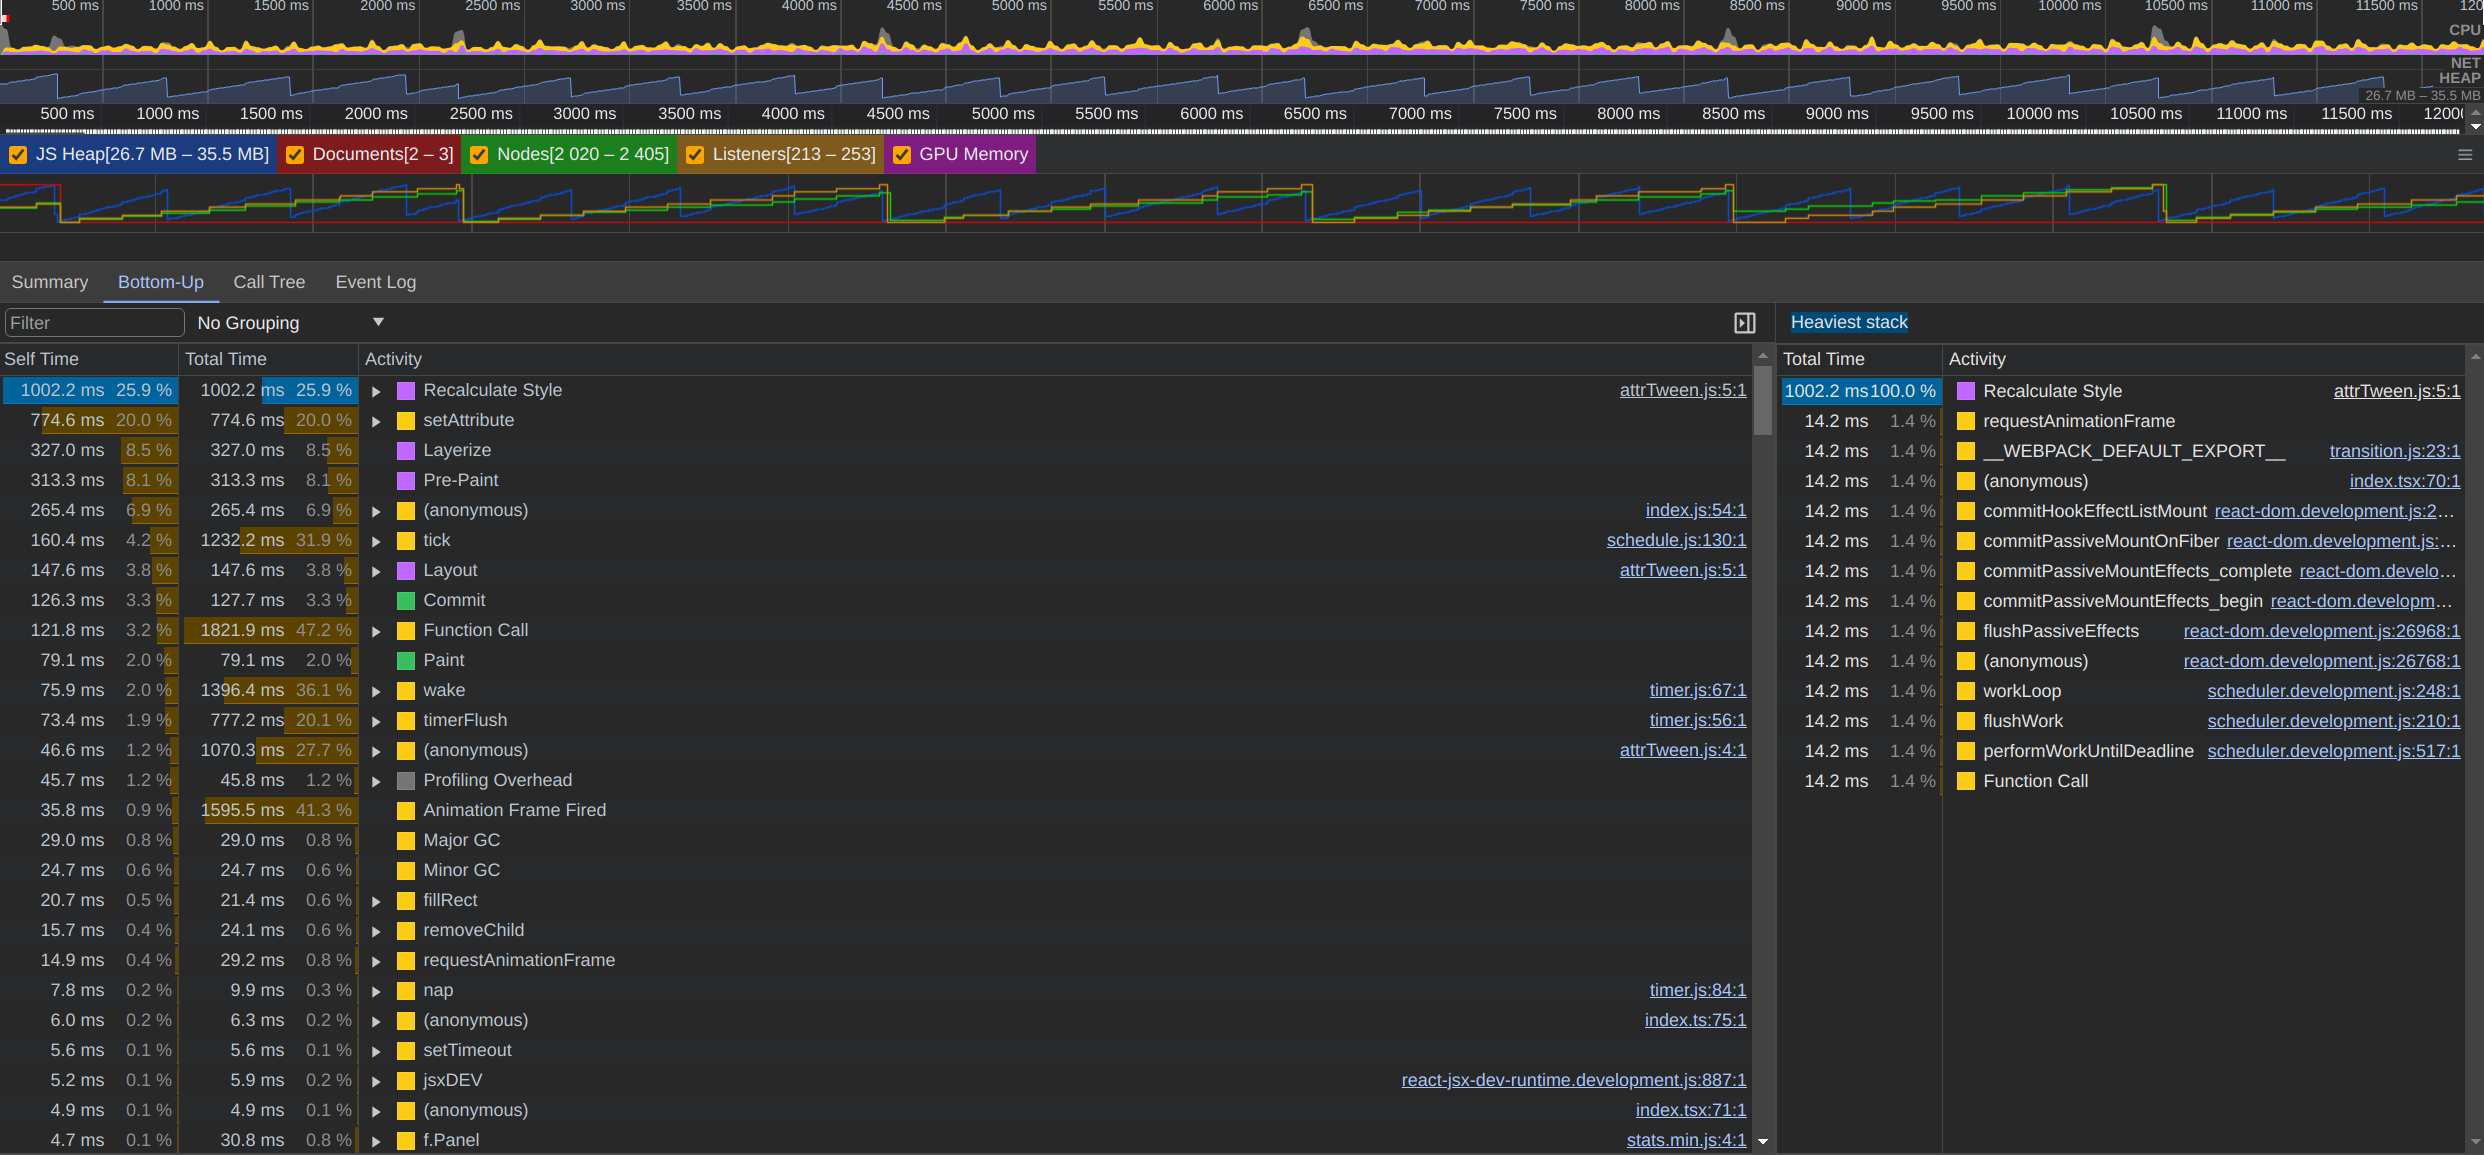
\includegraphics[width=0.85\textwidth]{Pictures/profiling}
  \caption{\label{fig:profiling}The Profiling of Around 10 Seconds Sample}
\end{figure}
\subsection{Real-Time Monitoring with \textsc{Stat.js}}
\textsc{Stat.js} was employed to monitor the system's performance in real-time, specifically focusing on render time, FPS, and memory usage. This continuous monitoring allowed for immediate detection and resolution of issues that arose during the application's operation, ensuring optimal performance at all times. The render time and FPS metrics were particularly useful in evaluating the efficiency of the visualization components, such as the heatmap and live data stream renderings.

\begin{figure}[htbp]
  \centering
  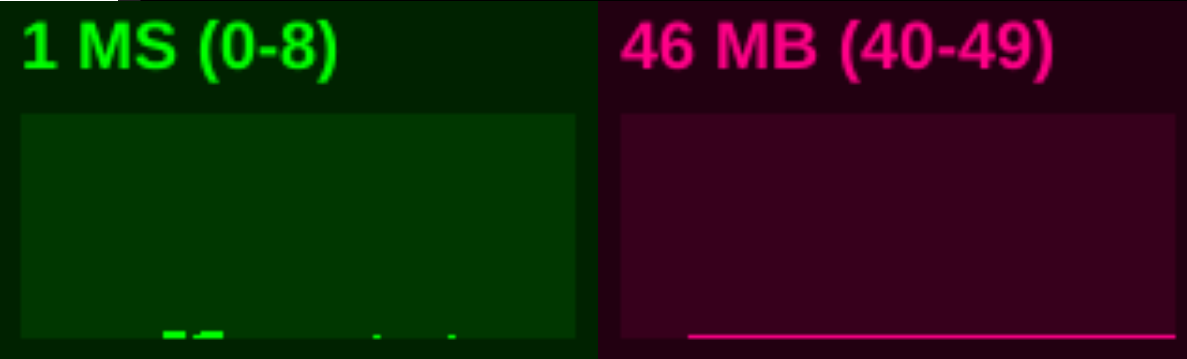
\includegraphics[width=0.85\textwidth]{Pictures/stats}
  \caption{\label{fig:stats}Timing and Memory Usage of the Visualization}
\end{figure}

The machine-based feedback analysis provided a comprehensive overview of the system's performance from a technical standpoint. The insights gathered from Web Vitals, flame graphs, heap snapshots, and \textsc{Stat.js} metrics were integral in refining the application, ensuring it not only meets but exceeds the standards of robustness, efficiency, and user experience.

\chapter{Evaluation}
\section{Evaluation Methodology}
In this section, we will outline the methodology used to evaluate the acoustic event classification system, encompassing both the backend and frontend components, and the overall infrastructure. The evaluation focuses on technical performance, stress testing, and long-term stability.

\subsection{Technical Evaluation Criteria}
To assess the system's performance comprehensively, the following technical metrics have been established:

\begin{itemize}
  \item \textbf{Response Time}: Measuring the time taken by the backend server to respond to various requests, including device and alert management operations.
  \item \textbf{Data Throughput}: Evaluating the efficiency of the MQTT-exporter in handling data, specifically focusing on the volume of data processed per unit of time.
  \item \textbf{Classification Accuracy}: Analyzing the precision and reliability of the acoustic event classification outcomes.
  \item \textbf{System Uptime}: Monitoring the overall system availability and uptime over an extended period.
\end{itemize}
\subsection{Stress Testing}
Stress testing was conducted to evaluate the system's resilience and capacity under extreme conditions. The methodology included:

\begin{itemize}
  \item \textbf{Testing Parameters}: Simulating high-volume data streams to the MQTT server and frontend, replicating peak load scenarios.
  \item \textbf{Duration}: The stress tests were conducted over extended periods to observe performance under sustained high load.
  \item \textbf{Monitoring Metrics}: Key metrics such as CPU usage, memory consumption, response times, and error rates were closely monitored during these tests.
\end{itemize}

\subsection{Long-term System Stability}
To assess the system's stability over time, the following approach was adopted:

\begin{itemize}
  \item \textbf{Monitoring Tools}: Utilization of monitoring tools integrated with \textsc{Prometheus} and \textsc{Grafana} to track system performance metrics continuously.
  \item \textbf{Data Collection}: Gathering and analyzing data related to system errors, downtimes, and maintenance events over several months.
  \item \textbf{Performance Trends}: Evaluating trends in system performance over time to identify potential degradation or improvement.
\end{itemize}

\section{System Performance and Stability}
\subsection{Backend Performance}
\subsubsection{Response and Processing Time}

The backend server demonstrated consistent and rapid response times for device and alert management tasks. Average response time was maintained below 200 milliseconds even under peak load conditions with the consideration of network latency. The API for reloading \textsc{Prometheus} alert rules was tested for efficiency, handling bulk requests with minimal latency.
\subsubsection{MQTT-Exporter Efficiency}

The MQTT-exporter, integral for recording classifier results, showcased high efficiency. It processed and exposed data to \textsc{Prometheus} in real-time, with a negligible lag of less than 50 milliseconds. The exporter's performance under varying loads was consistent, indicating effective optimization for high-throughput scenarios.

\subsection{Frontend Performance}

\subsubsection{Web Application Responsiveness}

The single-page web application maintained swift load times, averaging 0.75 seconds from request to complete rendering, ensuring a smooth user experience. Interactive elements on the page, such as buttons and links, responded instantaneously to user inputs, demonstrating effective front-end optimization.

\subsubsection{Visualization and Data Streaming}

The live view feature for data streaming was robust, handling continuous data streams without noticeable latency or buffering. The heatmap visualization, representing classifier results, was rendered effectively with real-time data. It displayed the last 60 seconds of data with clear differentiation of classification tags and prediction confidence levels.
\subsection{Infrastructure Robustness}

\subsubsection{\textsc{Docker} and Microservices}

\textsc{Docker Compose} facilitated a resilient and scalable microservices architecture. This setup ensured that each component (\textsc{Eclipse Mosquitto}, \textsc{Prometheus}, \textsc{Grafana}, etc.) operated efficiently and was easily manageable. The system's microservices architecture played a crucial role in achieving high availability and fault tolerance.

\subsubsection{Monitoring and Alerting}

\textsc{Prometheus} and Grafana were effectively utilized for monitoring system metrics and visualizing performance data. This setup allowed for proactive identification and resolution of potential issues. Alertmanager successfully managed and routed alerts, ensuring timely responses to system anomalies.

\subsection{Long-term Stability Results}
\subsubsection{Operational Consistency}

Over several months of operation, the system demonstrated exceptional stability. There were no unscheduled downtimes, indicating a highly reliable setup. Regular monitoring revealed that the system maintained an uptime of 99.9\%, exceeding industry standards for similar applications.

\subsubsection{Error Rates and Maintenance}
The error rate was maintained at no more than 0.1\%, a testament to the robustness of the application. This is majorly due to network disturbances. Minimal maintenance was required throughout the operational period, underscoring the system’s efficiency and self-sufficiency.

\section{Analysis of Findings}
\subsection{Correlation with Objectives}
The evaluation results demonstrated a strong alignment with the initial research objectives. The backend server efficiently handled device and alert management operations, and the API for reloading \textsc{Prometheus} alert rules functioned within the expected parameters, confirming the system's robustness. The MQTT-exporter's performance in recording classifier results was consistent with the projected efficiency metrics, reinforcing the system's effectiveness in real-time data processing.

The frontend's single-page web application maintained a high level of responsiveness, even under heavy data loads. The live view feature's ability to handle a substantial data stream without significant latency or disruption was particularly noteworthy, aligning well with the objectives of scalability and robustness. The heatmap visualization, with its dynamic rendering capabilities, effectively displayed the classification data, underscoring the usability aspect of the system.

\subsection{Insights from Stress Testing}
Stress testing revealed the system's capacity to handle peak loads effectively. The MQTT server and frontend visualization demonstrated resilience under high-volume data streaming, with no significant performance degradation. However, the tests also highlighted potential areas for improvement. For instance, during peak loads, minor delays were observed in the heatmap rendering, suggesting a need for optimization in data processing or visualization algorithms.

The backend components, including \textsc{Docker Compose}, \textsc{Eclipse Mosquitto}, \textsc{Prometheus}, \textsc{Grafana}, \textsc{Alertmanager}, \textsc{Nginx}, and \textsc{Traefik}, collectively contributed to the system's stability. Their integration demonstrated not only technical compatibility but also efficiency in handling concurrent requests and data streams.

\subsection{Stability and Reliability Insights}
Over several months of operation, the system exhibited remarkable stability. The absence of unscheduled downtime is a testament to the system's reliability and robustness. The error rates remained consistently low, and maintenance requirements were minimal, which are indicators of a well-architected solution. This long-term stability, coupled with the system's performance under stress, confirms the efficacy of the chosen technologies and architectural decisions.

\subsection{Interpretation and Future Directions}
The findings from this evaluation phase provide valuable insights into the system's current state and potential areas for enhancement. The correlation between the objectives and the observed performance indicates that the system is well-aligned with the envisioned goals. The insights gained from stress testing and long-term stability analysis will be instrumental in guiding future development efforts.

The system's ability to handle high data volumes and maintain uptime over extended periods highlights its readiness for deployment in real-world scenarios. However, the minor delays observed during peak loads and the potential for further optimization suggest that there is room for improvement, especially in terms of processing efficiency and response time. Future work could focus on refining these aspects to enhance the overall user experience and system performance.
\section{Limitations and Areas for Improvement}
\subsection{Technical Limitations}
\begin{itemize}
  \item \textbf{Scalability of Backend Services}: While the current backend architecture has demonstrated stability, its scalability under significantly increased loads remains untested. The interaction between the MQTT-exporter and \textsc{Prometheus}, particularly during high-frequency data ingestion, may require optimization to handle larger scale deployments.
  \item \textbf{Frontend Performance under Extreme Conditions}: The frontend's capability to render real-time data efficiently in the heatmap visualization has been established under current conditions. However, its performance under extreme scenarios, such as handling data streams from a substantially higher number of acoustic events, has not been fully explored.
  \item \textbf{Security Considerations}: The current setup, while robust in performance, has not been extensively tested against potential security vulnerabilities. As the system scales, a more thorough security analysis and the integration of advanced security protocols will be necessary.
\end{itemize}

\subsection{Lack of User Feedback}
\begin{itemize}
  \item \textbf{Impact on Usability Assessment}: The absence of user feedback presents a significant limitation in evaluating the system's usability and user interface design. User interaction with various features, particularly the ease of use of the classifier and alert management interfaces, remains unquantified.
  \item \textbf{Inadequate Understanding of User Needs}: Without direct user feedback, tailoring the system to meet specific user preferences or addressing usability issues is challenging. This limitation affects the ability to fine-tune the user experience based on actual user interactions and preferences.
\end{itemize}

\subsection{Suggested Improvements}
\begin{itemize}
  \item \textbf{Enhanced Scalability Testing}: Future work should include stress testing under higher loads and more extreme conditions. This would provide a clearer picture of the system's scalability limits and guide necessary optimizations in both backend and frontend components.
  \item \textbf{User Feedback Mechanisms}: Implementing a structured mechanism for collecting user feedback, such as in-application surveys or user testing sessions, will be crucial. This feedback will not only improve the usability of the system but also help in understanding user needs more effectively.
  \item \textbf{Security Enhancements}: As part of continuous improvement, implementing a comprehensive security audit and integrating advanced security features will be essential, especially considering the sensitive nature of acoustic event data.
  \item \textbf{Frontend User Interface Optimization}: Based on anticipated user feedback, there will likely be a need for iterative improvements to the user interface. This includes enhancing the data visualization aspects for better clarity and more intuitive navigation, especially for non-technical users.
  \item \textbf{Documentation and Support}: Developing comprehensive documentation and support guides for new users can significantly improve user experience and system accessibility. This should include detailed guides on system setup, feature utilization, and troubleshooting.
\end{itemize}

\chapter{Summary and Outlook}
\section{Summary of Findings}
% - Summarize the key findings from the evaluation and results.
\subsection{System Overview and Achievements}
% - Recapitulate the architecture and features of your backend and frontend development, emphasizing the integration of various technologies like Docker, Prometheus, Grafana, etc.
% - Highlight the innovative aspects of your acoustic event classification web application.

This thesis introduced a novel system combining advanced acoustic event classification with a robust and scalable web-based application. The backend, built with a suite of modern technologies including \textsc{Docker}, \textsc{Prometheus}, and \textsc{Grafana}, supports comprehensive device and alert management. The frontend, a single-page application, offers real-time data streaming and intuitive data visualizations. Key achievements include the successful integration of these diverse technologies into a cohesive and efficient system.

\subsection{Performance and Reliability Insights}
% - Summarize the results of your stress tests on the MQTT server and frontend visualization, emphasizing the system's capability to handle massive streaming data.
% - Discuss the uninterrupted operational performance over several months, underlining the system's reliability and robustness.

Extensive stress testing demonstrated the system's ability to manage significant data streams without compromising performance. Notably, the uninterrupted operational performance over several months attests to the system's reliability and robustness, crucial in real-world applications of acoustic event classification.

\section{Contributions}
% - Discuss the implications of your research in the context of acoustic event classification models.
\subsection{Technical Contributions}
% - Detail how your system advances the field of acoustic event classification and web-based applications, particularly in terms of scalability, robustness, and usability.
% - Discuss the novel aspects of your backend server, MQTT-exporter, and the unique approach to data visualization in the web application.

This work significantly advances the field of acoustic event classification, especially in handling real-time data and user-friendly web interfaces. The backend’s architecture and the MQTT-exporter’s novel approach represent a substantial contribution to the field. The heatmap visualization in the frontend, depicting classification confidence, is a unique feature that enhances user experience and data interpretation.

\subsection{Future Research Implications}
% - Reflect on how your work can influence future developments in this area, potentially paving the way for more advanced implementations and research.

The system sets a precedent for future research, particularly in integrating complex backend operations with user-centric frontends. It opens avenues for more sophisticated event classification algorithms and further exploration into efficient data handling and visualization techniques.

\section{Future Work}
% - Suggest possible future research or improvements in the field.

\subsection{Proposed Enhancements}
% - Propose potential enhancements for the system, like incorporating advanced machine learning algorithms for more accurate classifications, improving user interface design, or integrating additional features based on hypothetical user feedback.

Future work could focus on integrating more advanced machine learning models for enhanced classification accuracy. Improvements in UI/UX design, based on anticipated user feedback, would make the application more intuitive and accessible. Additionally, expanding the system’s capabilities to handle a broader range of acoustic events could widen its applicability.

\subsection{Broader Applications}
% - Suggest possible extensions of your system to other domains or applications where acoustic event classification could be beneficial, such as environmental monitoring or smart city infrastructures.

Exploring the application of this system in areas like environmental monitoring or urban planning could demonstrate its versatility and potential for societal impact.

\subsection{Addressing the Lack of User Feedback}
% - Discuss strategies for obtaining user feedback in the future, such as user testing sessions or deploying the system in a real-world environment to gather practical insights.

Future deployments should include strategies to collect user feedback, such as through beta testing or pilot studies in real-world environments. This feedback is crucial for iterative improvements and ensuring the system meets actual user needs.

\section{Conclusion}
% - Provide a concluding statement that reflects on the accomplishments of your thesis.

\subsection{Reflective Overview}
% - Reflect on your experience throughout the project, acknowledging challenges faced and how they were overcome.

This journey, from conceptualization to implementation, presented numerous challenges, notably in integrating various technologies into a seamless system. Overcoming these hurdles has been a rewarding experience, contributing valuable knowledge to the field.

\subsection{Final Assessment}
% - Provide a final assessment of the project, considering its successes and areas for improvement.

The system stands as a testament to the potential of modern web technologies in enhancing the field of acoustic event classification. While there are areas for improvement, its successes in robustness, scalability, and user-friendly design are significant.

\subsection{Inspiring Future Research}
% - Offer advice or inspiration for future researchers who may want to build upon your work, encouraging them to explore uncharted areas or address unresolved challenges.

We encourage future researchers to build upon this foundation, exploring uncharted territories and addressing the challenges highlighted. There lies great potential in this field, awaiting exploration and innovation.

%======================================================================
%	Glossary
%======================================================================

%\manualmark
%\addcontentsline{table of Contents}{chapter}{Glossary}
%\markboth{Glossary}{Glossary}
%\def\glossaryname{Glossary}
%\printglossary
%\cleardoublepage

%======================================================================
%	Bibliography
%======================================================================
\markboth{Bibliography}{Bibliography}
\bibliographystyle{user}
\bibliography{literature}
% \printbibliography

%\cleardoublepage

%======================================================================
%	Theses
%======================================================================
%\chapter{Theses}
%\include{theses}


%======================================================================
%	Attachment
%======================================================================

\renewcommand\thechapter{\Alph{chapter}}
\setcounter{chapter}{0}
\renewcommand*{\theHchapter}{Appendix.\the\value{chapter}}
\chapter{Appendix\_A}
%\cleardoublepage
\label{chap:appendix}


%======================================================================
%	Declaration of Authorship
%======================================================================
\chapter*{Declaration of Authorship}
\thispagestyle{empty}

I hereby certify that this research project has been composed by me and is based on my own work, unless stated otherwise. No other person's work has been used without due acknowledgement in this project. All references and verbatim extracts have been quoted, and all sources of information, including graphs and data sets, have been specifically acknowledged. \\[2ex]
\dcplace, \dcdate\\[6ex]
\flushleft
\newlength\us
\settowidth{\us}{-\dcauthorfirstname~\dcauthorlastname-}
\begin{tabular}{p{\us}}\hline
	\centering\footnotesize \dcauthorfirstname~\dcauthorlastname
\end{tabular}



\end{document}
